\chapter{Results}
\label{sec:results}
\providecommand{\descriptionFakePhoton}[1]{\if d#1%
The data-driven estimate for \nonprompt photons is used%
\else
\Nonprompt photons are estimated from simulation%
\fi}

\providecommand{\captionScan}[5]{
Likelihood scan for the signal strength parameter
on the #1,
using the #2 working point of the photon #3.
\descriptionFakePhoton{#4}.
The FSR cut is #5applied.
The effect of groups of nuisance parameters on the uncertainty is assessed by sequentially fixing their value in the fit.
}
 % Template captions for results

In this chapter the results of
the measurement of the cross section of $\Pp\Pp \to 4\Pl \PGg$, as well as
the search for $\PZ\PZ\PGg$ triboson production are presented
in Sections~\ref{sec:results_4L_inclusive} and~\ref{sec:results_4L_FSRcut} respectively.
Preliminary results for the three lepton channel, focusing on the cross section of the $\Pp\Pp \to 3\Pl\PGnl\PGg$,
are also reported in Section~\ref{sec:results_3L}.
This analysis uses the data collected by the CMS experiment during the 2016--2018 period at a centre-of-mass energy of 13\TeV.
The analysis strategy is to search for excess events over the estimated background yield from known Standard Model processes.
Different identification strategies for the photon and several kinematic distributions are explored.

First the statistical tools used for the extraction of the parameters of interest and interpretation are described.
Then the expected result before unblinding is discussed, and the best strategy selected.
Finally, the observed results are shown.

\section{Yields and kinematic distributions}
\label{sec:yields}
After the selections described in Section \ref{sec:event_selection}, the event yields are extracted for signal and backgrounds for each of the four periods of \Run2, for the signal and control regions.

\subsection{Four lepton channel}
The pre-fit yields for the signal and background processes for the signal region
with four leptons passing the tight selection and a photon passing the cut-based ID (SR4P\_1P),
can be seen in Table \ref{tab:Run2_SR4P_phoCR_lepCR} (Table~\ref{tab:Run2_SR4P_phoMC_lepCR})
when using the data-driven (simulation) to estimate tha fake photon background.
Alternatively, the expected yields obtained using the
working point \texttt{wp90} of the MVA ID are shown in Table~\ref{tab:Run2_SR4P_phoMC_lepCR_wp90}.

Additional tables, including also the observed number of data events, are provided
for the fake photon application region (Table \ref{tab:yields_Run2_CR4P_1F_lepCR}),
and for the fake lepton application regions (Tables \ref{tab:yields_Run2_CR3P1F_1P} and \ref{tab:yields_Run2_CR2P2F_1P}).

The yields in the triboson fiducial region are shown
in Table~\ref{tab:yield_SR4P_1P_FSRcut_Loose} for the Loose working point of the cut-based ID,
and in Table~\ref{tab:yield_SR4P_1P_FSRcut_wp90} when using the \texttt{wp80} of the MVA ID instead.

\begin{table}
  \caption{Yields from the signal region SR4P\_1P, with four leptons passing the tight selection and a photon passing the cut-based ID.
  The \nonprompt and misidentified photons are estimated with the data-driven method
  and thus only the events containing a prompt generated photon are included from the main background samples.
  }
  \label{tab:Run2_SR4P_phoCR_lepCR}
  % Note: this is from the variable mZZGloose
  \resizebox{\textwidth}{!}{%
  \begin{tabular}{lccccc}
    \toprule
    {}                            & 2016preVFP         & 2016postVFP        & 2017               & 2018               & \Run2               \\
    \midrule
    $\PZ\PZ\PGg\to4\Pl\PGg$       &  1.962 $\pm$ 0.047 &  1.714 $\pm$ 0.040 &  4.021 $\pm$ 0.100 &  5.864 $\pm$ 0.142 &  13.561 $\pm$ 0.184 \\
    $\Pg\Pg\to\PZ\PZ\to4\Pe$      &  0.031 $\pm$ 0.001 &  0.030 $\pm$ 0.001 &  0.076 $\pm$ 0.002 &  0.104 $\pm$ 0.003 &   0.240 $\pm$ 0.004 \\
    $\Pg\Pg\to\PZ\PZ\to2\Pe2\PGm$ &  0.063 $\pm$ 0.003 &  0.057 $\pm$ 0.002 &  0.069 $\pm$ 0.003 &  0.104 $\pm$ 0.004 &   0.292 $\pm$ 0.006 \\
    $\Pg\Pg\to\PZ\PZ\to4\PGm$     &  0.056 $\pm$ 0.001 &  0.046 $\pm$ 0.001 &  0.117 $\pm$ 0.003 &  0.159 $\pm$ 0.004 &   0.378 $\pm$ 0.005 \\
    $\PZ\PZ\PZ$                   &  0.007 $\pm$ 0.005 &  0.000 $\pm$ 0.000 &  0.017 $\pm$ 0.008 &  0.029 $\pm$ 0.010 &   0.053 $\pm$ 0.014 \\
    $\PQt\PAQt\PZ$+jets           &  0.011 $\pm$ 0.002 &  0.010 $\pm$ 0.002 &  0.036 $\pm$ 0.005 &  0.041 $\pm$ 0.006 &   0.098 $\pm$ 0.009 \\
    Fake photons                  &  1.357 $\pm$ 0.655 &  1.011 $\pm$ 0.509 &  1.368 $\pm$ 0.519 &  2.451 $\pm$ 0.691 &   6.187 $\pm$ 1.198 \\
    $\PW\PZ\PZ$                   &  0.000 $\pm$ 0.000 &  0.021 $\pm$ 0.012 &  0.016 $\pm$ 0.015 &  0.065 $\pm$ 0.027 &   0.102 $\pm$ 0.033 \\
    $\PW\PW\PZ$                   &  0.000 $\pm$ 0.000 &  0.040 $\pm$ 0.040 &  0.041 $\pm$ 0.041 &  0.082 $\pm$ 0.058 &   0.163 $\pm$ 0.082 \\
    \noalign{\vspace{.3ex}}\hline\noalign{\vspace{.3ex}}
    Total                         &  3.488 $\pm$ 0.656 &  2.927 $\pm$ 0.512 &  5.759 $\pm$ 0.531 &  8.900 $\pm$ 0.709 &  21.074 $\pm$ 1.215 \\
    \bottomrule
  \end{tabular}
  }
\end{table}

\begin{table}
  \caption{Yields from the signal region SR4P\_1P, with four leptons passing the tight selection and a photon passing the cut-based ID.
    The \nonprompt and misidentified photons are taken from the simulation.
  }
  \label{tab:Run2_SR4P_phoMC_lepCR}
  % Note: this is from the variable mZZGloose
  \resizebox{\textwidth}{!}{%
  \begin{tabular}{lccccc}
    \toprule
    {}                            & 2016preVFP          & 2016postVFP       & 2017               & 2018               & \Run2               \\
    \midrule
    $\PZ\PZ\PGg\to4\Pl\PGg$       &  1.962 $\pm$ 0.047 &  1.714 $\pm$ 0.040 &  4.021 $\pm$ 0.100 &  5.864 $\pm$ 0.142 &  13.561 $\pm$ 0.184 \\
    $\PQq\PAQq\to\PZ\PZ\to4\Pl$   &  0.243 $\pm$ 0.011 &  0.210 $\pm$ 0.009 &  0.610 $\pm$ 0.018 &  0.858 $\pm$ 0.025 &   1.921 $\pm$ 0.034 \\
    $\Pg\Pg\to\PZ\PZ\to4\Pe$      &  0.036 $\pm$ 0.001 &  0.035 $\pm$ 0.001 &  0.088 $\pm$ 0.002 &  0.124 $\pm$ 0.003 &   0.283 $\pm$ 0.004 \\
    $\Pg\Pg\to\PZ\PZ\to2\Pe2\PGm$ &  0.077 $\pm$ 0.003 &  0.070 $\pm$ 0.003 &  0.086 $\pm$ 0.003 &  0.127 $\pm$ 0.005 &   0.360 $\pm$ 0.007 \\
    $\Pg\Pg\to\PZ\PZ\to4\PGm$     &  0.065 $\pm$ 0.001 &  0.054 $\pm$ 0.001 &  0.139 $\pm$ 0.003 &  0.192 $\pm$ 0.005 &   0.449 $\pm$ 0.006 \\
    $\PZ\PZ\PZ$                   &  0.007 $\pm$ 0.005 &  0.003 $\pm$ 0.003 &  0.021 $\pm$ 0.009 &  0.050 $\pm$ 0.014 &   0.082 $\pm$ 0.017 \\
    $\PW\PZ\PZ$                   &  0.008 $\pm$ 0.008 &  0.028 $\pm$ 0.014 &  0.038 $\pm$ 0.020 &  0.088 $\pm$ 0.031 &   0.163 $\pm$ 0.041 \\
    $\PQt\PAQt\PZ$+jets           &  0.012 $\pm$ 0.003 &  0.011 $\pm$ 0.002 &  0.048 $\pm$ 0.006 &  0.054 $\pm$ 0.007 &   0.124 $\pm$ 0.010 \\
    Fake leptons                  &  0.047 $\pm$ 0.066 &  0.000 $\pm$ 0.000 &  0.089 $\pm$ 0.119 &  0.117 $\pm$ 0.091 &   0.253 $\pm$ 0.164 \\
    $\PW\PW\PZ$                   &  0.000 $\pm$ 0.000 &  0.040 $\pm$ 0.040 &  0.041 $\pm$ 0.041 &  0.082 $\pm$ 0.058 &   0.163 $\pm$ 0.082 \\
    Total                         &  2.458 $\pm$ 0.082 &  2.164 $\pm$ 0.059 &  5.181 $\pm$ 0.164 &  7.557 $\pm$ 0.183 &  17.360 $\pm$ 0.266 \\
    \noalign{\vspace{.3ex}}\hline\noalign{\vspace{.3ex}}
    Total                         &  3.488 $\pm$ 0.656 &  2.927 $\pm$ 0.512 &  5.759 $\pm$ 0.531 &  8.900 $\pm$ 0.709 &  21.074 $\pm$ 1.215 \\
    \bottomrule
  \end{tabular}
  }
\end{table}

\begin{table}
  \caption{Yields from the signal region SR4P\_1P, with four leptons passing the tight selection
  and a photon passing the \texttt{wp90} of the MVA based ID.
  The \nonprompt and misidentified photons are taken from the simulation.
  }
  \label{tab:Run2_SR4P_phoMC_lepCR_wp90}
  % Note: this is from the variable mZZGloose
  \resizebox{\textwidth}{!}{%
  \begin{tabular}{lccccc}
    \toprule
    {}                            & 2016preVFP          & 2016postVFP       & 2017               & 2018               & \Run2               \\
    \midrule
    $\PZ\PZ\PGg\to4\Pl\PGg$       &  2.026 $\pm$ 0.047 &  1.781 $\pm$ 0.041 &  4.294 $\pm$ 0.103 &  6.126 $\pm$ 0.143 & 14.227 $\pm$ 0.187 \\
    $\PQq\PAQq\to\PZ\PZ\to4\Pl$   &  0.192 $\pm$ 0.009 &  0.158 $\pm$ 0.008 &  0.452 $\pm$ 0.015 &  0.652 $\pm$ 0.022 &  1.453 $\pm$ 0.029 \\
    $\Pg\Pg\to\PZ\PZ\to4\Pe$      &  0.036 $\pm$ 0.001 &  0.034 $\pm$ 0.001 &  0.090 $\pm$ 0.002 &  0.120 $\pm$ 0.003 &  0.280 $\pm$ 0.004 \\
    $\Pg\Pg\to\PZ\PZ\to2\Pe2\PGm$ &  0.076 $\pm$ 0.003 &  0.068 $\pm$ 0.003 &  0.086 $\pm$ 0.003 &  0.131 $\pm$ 0.005 &  0.361 $\pm$ 0.007 \\
    $\Pg\Pg\to\PZ\PZ\to4\PGm$     &  0.066 $\pm$ 0.001 &  0.053 $\pm$ 0.001 &  0.141 $\pm$ 0.003 &  0.189 $\pm$ 0.004 &  0.449 $\pm$ 0.006 \\
    $\PZ\PZ\PZ$                   &  0.010 $\pm$ 0.006 &  0.003 $\pm$ 0.003 &  0.023 $\pm$ 0.009 &  0.040 $\pm$ 0.012 &  0.076 $\pm$ 0.016 \\
    $\PQt\PAQt\PZ$+jets           &  0.014 $\pm$ 0.003 &  0.012 $\pm$ 0.002 &  0.045 $\pm$ 0.006 &  0.057 $\pm$ 0.007 &  0.129 $\pm$ 0.010 \\
    Fake leptons                  &  0.045 $\pm$ 0.066 &  0.103 $\pm$ 0.117 &  0.107 $\pm$ 0.118 &  0.022 $\pm$ 0.081 &  0.276 $\pm$ 0.196 \\
    $\PW\PZ\PZ$                   &  0.000 $\pm$ 0.000 &  0.020 $\pm$ 0.012 &  0.063 $\pm$ 0.022 &  0.076 $\pm$ 0.029 &  0.159 $\pm$ 0.038 \\
    $\PW\PW\PZ$                   &  0.000 $\pm$ 0.000 &  0.000 $\pm$ 0.000 &  0.040 $\pm$ 0.040 &  0.080 $\pm$ 0.057 &  0.121 $\pm$ 0.070 \\
    \noalign{\vspace{.3ex}}\hline\noalign{\vspace{.3ex}}
    Total                         &  2.464 $\pm$ 0.082 &  2.233 $\pm$ 0.124 &  5.342 $\pm$ 0.165 &  7.493 $\pm$ 0.178 & 17.532 $\pm$ 0.285 \\
    \bottomrule
  \end{tabular}
  }
\end{table}

\begin{table}
\caption{Yields from the fake photon application region CR4P\_1F, with four leptons passing the tight selection and a photon passing the VeryLoose ID but failing the cut-based ID Loose.}
\label{tab:yields_Run2_CR4P_1F_lepCR}
\resizebox{\textwidth}{!}{%
  \begin{tabular}{lccccc}
    \toprule
    {}                            & 2016preVFP         & 2016postVFP        & 2017               & 2018                & \Run2               \\
    \midrule
    $\PZ\PZ\PGg\to4\Pl\PGg$       &  0.302 $\pm$ 0.019 &  0.294 $\pm$ 0.017 &  0.837 $\pm$ 0.047 &   1.191 $\pm$ 0.064 &   2.623 $\pm$ 0.083 \\
    $\PQq\PAQq\to\PZ\PZ\to4\Pl$   &  2.400 $\pm$ 0.033 &  2.283 $\pm$ 0.030 &  6.428 $\pm$ 0.058 &   9.507 $\pm$ 0.084 &  20.617 $\pm$ 0.111 \\
    $\Pg\Pg\to\PZ\PZ\to4\Pe$      &  0.060 $\pm$ 0.001 &  0.059 $\pm$ 0.001 &  0.168 $\pm$ 0.003 &   0.258 $\pm$ 0.005 &   0.546 $\pm$ 0.006 \\
    $\Pg\Pg\to\PZ\PZ\to2\Pe2\PGm$ &  0.157 $\pm$ 0.004 &  0.158 $\pm$ 0.004 &  0.224 $\pm$ 0.005 &   0.322 $\pm$ 0.008 &   0.860 $\pm$ 0.011 \\
    $\Pg\Pg\to\PZ\PZ\to4\PGm$     &  0.107 $\pm$ 0.002 &  0.092 $\pm$ 0.002 &  0.253 $\pm$ 0.004 &   0.385 $\pm$ 0.006 &   0.837 $\pm$ 0.008 \\
    $\PZ\PZ\PZ$                   &  0.039 $\pm$ 0.011 &  0.025 $\pm$ 0.011 &  0.067 $\pm$ 0.016 &   0.069 $\pm$ 0.019 &   0.200 $\pm$ 0.030 \\
    $\PW\PZ\PZ$                   &  0.064 $\pm$ 0.022 &  0.071 $\pm$ 0.023 &  0.120 $\pm$ 0.034 &   0.120 $\pm$ 0.038 &   0.376 $\pm$ 0.060 \\
    $\PW\PW\PZ$                   &  0.048 $\pm$ 0.048 &  0.046 $\pm$ 0.046 &  0.000 $\pm$ 0.000 &   0.036 $\pm$ 0.036 &   0.131 $\pm$ 0.076 \\
    $\PQt\PAQt\PZ$+jets           &  0.056 $\pm$ 0.006 &  0.050 $\pm$ 0.005 &  0.171 $\pm$ 0.011 &   0.253 $\pm$ 0.015 &   0.530 $\pm$ 0.020 \\
    Fake leptons                  &  0.030 $\pm$ 0.052 &  0.051 $\pm$ 0.047 &  0.059 $\pm$ 0.092 &   0.050 $\pm$ 0.095 &   0.191 $\pm$ 0.149 \\
    \noalign{\vspace{.3ex}}\hline\noalign{\vspace{.3ex}}
    Total                         &  3.263 $\pm$ 0.084 &  3.130 $\pm$ 0.078 &  8.327 $\pm$ 0.124 &  12.191 $\pm$ 0.154 &  26.911 $\pm$ 0.229 \\
    Data                          &  5                 &  4                 &  7                 &  13                 &  29                 \\
    \bottomrule
  \end{tabular}
  }
\end{table}

\begin{table}
\caption{Yields in CR3P1F\_1P, one of the fake lepton application regions, with three leptons passing the tight selection, one passing only a loose selection, and a photon passing the cut-based ID.}
\label{tab:yields_Run2_CR3P1F_1P}
\resizebox{\textwidth}{!}{%
  \begin{tabular}{lccccc}
  \toprule
  {}                            & 2016preVFP          & 2016postVFP       & 2017               & 2018               & \Run2              \\
  \midrule
  $\PZ\PZ\PGg\to4\Pl\PGg$       &  0.143 $\pm$ 0.013 &  0.139 $\pm$ 0.011 &  0.390 $\pm$ 0.031 &  0.506 $\pm$ 0.041 &  1.178 $\pm$ 0.055 \\
  $\PW\PZ\PGg\to3\Pl\PGnl\PGg$  &  0.213 $\pm$ 0.011 &  0.191 $\pm$ 0.008 &  0.415 $\pm$ 0.020 &  0.711 $\pm$ 0.030 &  1.530 $\pm$ 0.039 \\
  $\PZ\PGg\to\Pl\Pl\PGg$        &  0.750 $\pm$ 0.285 &  0.000 $\pm$ 0.000 &  0.463 $\pm$ 0.388 &  0.492 $\pm$ 0.447 &  1.705 $\pm$ 0.657 \\
  $\PQq\PAQq\to\PZ\PZ\to4\Pl$   &  0.103 $\pm$ 0.007 &  0.085 $\pm$ 0.006 &  0.235 $\pm$ 0.011 &  0.328 $\pm$ 0.016 &  0.751 $\pm$ 0.021 \\
  $\Pg\Pg\to\PZ\PZ\to4\Pe$      &  0.011 $\pm$ 0.001 &  0.008 $\pm$ 0.000 &  0.022 $\pm$ 0.001 &  0.037 $\pm$ 0.002 &  0.078 $\pm$ 0.002 \\
  $\Pg\Pg\to\PZ\PZ\to2\Pe2\PGm$ &  0.012 $\pm$ 0.001 &  0.012 $\pm$ 0.001 &  0.016 $\pm$ 0.001 &  0.022 $\pm$ 0.002 &  0.062 $\pm$ 0.003 \\
  $\Pg\Pg\to\PZ\PZ\to4\PGm$     &  0.003 $\pm$ 0.000 &  0.003 $\pm$ 0.000 &  0.007 $\pm$ 0.001 &  0.008 $\pm$ 0.001 &  0.020 $\pm$ 0.001 \\
  $\PW\PZ\to3\Pl\PGn$           &  0.047 $\pm$ 0.027 &  0.035 $\pm$ 0.027 &  0.135 $\pm$ 0.087 &  1.101 $\pm$ 0.319 &  1.317 $\pm$ 0.333 \\
  $\PZ\PZ\PZ$                   &  0.003 $\pm$ 0.003 &  0.000 $\pm$ 0.000 &  0.010 $\pm$ 0.006 &  0.007 $\pm$ 0.005 &  0.020 $\pm$ 0.008 \\
  $\PW\PZ\PZ$                   &  0.009 $\pm$ 0.009 &  0.000 $\pm$ 0.000 &  0.001 $\pm$ 0.012 &  0.012 $\pm$ 0.012 &  0.022 $\pm$ 0.019 \\
  $\PQt\PAQt\PZ$+jets           &  0.043 $\pm$ 0.005 &  0.039 $\pm$ 0.004 &  0.068 $\pm$ 0.007 &  0.114 $\pm$ 0.010 &  0.263 $\pm$ 0.014 \\
  Drell-Yan + jets              &  0.000 $\pm$ 0.000 &  0.000 $\pm$ 0.000 &  0.000 $\pm$ 0.000 &  0.680 $\pm$ 3.520 &  0.680 $\pm$ 3.520 \\
  \noalign{\vspace{.3ex}}\hline\noalign{\vspace{.3ex}}
  Total                         &  1.337 $\pm$ 0.287 &  0.512 $\pm$ 0.031 &  1.760 $\pm$ 0.399 &  4.017 $\pm$ 3.563 &  7.625 $\pm$ 3.597 \\
  Data                          &  1.000 $\pm$ 1.000 &  0.000 $\pm$ 0.000 &  2.000 $\pm$ 1.414 &  5.000 $\pm$ 2.236 &  8.000 $\pm$ 2.828 \\
  \bottomrule
  \end{tabular}
  }
\end{table}

\begin{table}
\caption{Yields in CR2P2F\_1P, one of the fake lepton application regions, with two leptons passing the tight selection, two passing only a loose selection, and a photon passing the cut-based ID.}
\label{tab:yields_Run2_CR2P2F_1P}
\resizebox{\textwidth}{!}{%
  \begin{tabular}{lccccc}
    \toprule
    {} & 2016preVFP & 2016postVFP & 2017 & 2018 & Run2 \\
    \midrule
    $\PZ\PZ\PGg\to4\Pl\PGg$      &   0.009 $\pm$ 0.004 &  0.005 $\pm$ 0.002 &   0.006 $\pm$ 0.004 &    0.034 $\pm$ 0.010 &    0.054 $\pm$ 0.012 \\
    $\PW\PZ\PGg\to3\Pl\PGnl\PGg$ &   0.023 $\pm$ 0.003 &  0.020 $\pm$ 0.003 &   0.034 $\pm$ 0.006 &    0.053 $\pm$ 0.008 &    0.130 $\pm$ 0.011 \\
    Drell-Yan + jets             &   6.231 $\pm$ 3.599 &  1.855 $\pm$ 1.855 &  15.810 $\pm$ 5.603 &  37.763 $\pm$ 15.469 &  61.659 $\pm$ 16.943 \\
    $\PZ\PGg\to\Pl\Pl\PGg$       &   6.600 $\pm$ 0.799 &  0.000 $\pm$ 0.000 &  13.784 $\pm$ 1.461 &   22.222 $\pm$ 2.340 &   42.606 $\pm$ 2.872 \\
    $\PQq\PAQq\to\PZ\PZ\to4\Pl$  &   0.009 $\pm$ 0.002 &  0.007 $\pm$ 0.002 &   0.015 $\pm$ 0.003 &    0.023 $\pm$ 0.004 &    0.054 $\pm$ 0.006 \\
    $\PW\PZ\to3\Pl\PGnl$         &   0.002 $\pm$ 0.022 &  0.027 $\pm$ 0.019 &   0.123 $\pm$ 0.075 &    0.151 $\pm$ 0.136 &    0.302 $\pm$ 0.158 \\
    $\PQt\PAQt\PZ$+jets          &   0.023 $\pm$ 0.004 &  0.020 $\pm$ 0.003 &   0.035 $\pm$ 0.005 &    0.055 $\pm$ 0.007 &    0.133 $\pm$ 0.010 \\
    $\PQt\PZ\PQq$                &   0.005 $\pm$ 0.008 &  0.001 $\pm$ 0.006 &   0.018 $\pm$ 0.009 &    0.024 $\pm$ 0.013 &    0.048 $\pm$ 0.019 \\
    $\PQt\PW$                    &   0.057 $\pm$ 0.057 &  0.000 $\pm$ 0.000 &   0.088 $\pm$ 0.099 &    0.000 $\pm$ 0.000 &    0.144 $\pm$ 0.114 \\
    \noalign{\vspace{.3ex}}\hline\noalign{\vspace{.3ex}}
    Total                        &   6.616 $\pm$ 0.789 & 11.123 $\pm$ 6.842 & 28.359 $\pm$ 10.849 &  50.717 $\pm$ 14.889 &  96.814 $\pm$ 19.667 \\
    Data                         &  17                 &  9                 & 23                  &  28                  &  77                  \\
    \bottomrule
  \end{tabular}
  }
\end{table}

\begin{table}
  \caption{Yields in the fiducial triboson region of the four lepton channel, using the cut-based ID selection for the photon.}
  \label{tab:yield_SR4P_1P_FSRcut_Loose}
  \resizebox{\textwidth}{!}{%
  \begin{tabular}{lrrrrr}
    \toprule
    {}                           & 2016preVFP         & 2016postVFP        & 2017               & 2018               & \Run2              \\
    \midrule
    $\PZ\PZ\PGg\to4\Pl\PGg$      &  0.841 $\pm$ 0.031 &  0.728 $\pm$ 0.026 &  1.761 $\pm$ 0.066 &  2.485 $\pm$ 0.093 &  5.815 $\pm$ 0.121 \\
    $\PQq\PAQq\to\PZ\PZ\to4\Pl$  &  0.197 $\pm$ 0.010 &  0.167 $\pm$ 0.008 &  0.504 $\pm$ 0.016 &  0.701 $\pm$ 0.023 &  1.569 $\pm$ 0.031 \\
    Fake leptons                 &  0.064 $\pm$ 0.066 &  0.000 $\pm$ 0.000 &  0.106 $\pm$ 0.115 &  0.102 $\pm$ 0.086 &  0.272 $\pm$ 0.157 \\
    $\Pg\Pg\to\PZ\PZ\to4\PGm$    &  0.009 $\pm$ 0.001 &  0.010 $\pm$ 0.000 &  0.024 $\pm$ 0.001 &  0.036 $\pm$ 0.002 &  0.079 $\pm$ 0.002 \\
    $\Pg\Pg\to\PZ\PZ\to2\Pe2\PGm$&  0.021 $\pm$ 0.002 &  0.017 $\pm$ 0.001 &  0.023 $\pm$ 0.002 &  0.032 $\pm$ 0.002 &  0.094 $\pm$ 0.004 \\
    $\Pg\Pg\to\PZ\PZ\to4\Pe$     &  0.020 $\pm$ 0.001 &  0.016 $\pm$ 0.001 &  0.042 $\pm$ 0.002 &  0.060 $\pm$ 0.003 &  0.137 $\pm$ 0.003 \\
    $\PZ\PZ\PZ$                  &  0.004 $\pm$ 0.004 &  0.003 $\pm$ 0.003 &  0.014 $\pm$ 0.007 &  0.032 $\pm$ 0.011 &  0.052 $\pm$ 0.014 \\
    $\PW\PZ\PZ$                  &  0.000 $\pm$ 0.000 &  0.014 $\pm$ 0.010 &  0.023 $\pm$ 0.017 &  0.068 $\pm$ 0.028 &  0.106 $\pm$ 0.034 \\
    $\PQt\PAQt\PZ$+jets          &  0.005 $\pm$ 0.002 &  0.004 $\pm$ 0.001 &  0.022 $\pm$ 0.004 &  0.023 $\pm$ 0.005 &  0.055 $\pm$ 0.006 \\
    \noalign{\vspace{.3ex}}\hline\noalign{\vspace{.3ex}}
    Total                        &  1.160 $\pm$ 0.073 &  0.959 $\pm$ 0.030 &  2.520 $\pm$ 0.135 &  3.539 $\pm$ 0.132 &  8.178 $\pm$ 0.205 \\
    \bottomrule
  \end{tabular}
  }
\end{table}

\begin{table}
  \caption{Yields in the fiducial triboson region of the four lepton channel, using the \texttt{wp90} of the MVA ID selection for the photon.}
  \label{tab:yield_SR4P_1P_FSRcut_wp90}
  \resizebox{\textwidth}{!}{%
  \begin{tabular}{lrrrrr}
    \toprule
    {}                            & 2016preVFP         & 2016postVFP        & 2017               & 2018               & \Run2              \\
    \midrule
    $\PZ\PZ\PGg\to4\Pl\PGg$       &  0.804 $\pm$ 0.030 &  0.694 $\pm$ 0.025 &  1.703 $\pm$ 0.065 &  2.374 $\pm$ 0.089 &  5.576 $\pm$ 0.117 \\
    $\PQq\PAQq\to\PZ\PZ\to4\Pl$   &  0.088 $\pm$ 0.006 &  0.066 $\pm$ 0.005 &  0.209 $\pm$ 0.010 &  0.292 $\pm$ 0.014 &  0.656 $\pm$ 0.019 \\
    $\Pg\Pg\to\PZ\PZ\to4\Pe$      &  0.007 $\pm$ 0.000 &  0.007 $\pm$ 0.000 &  0.017 $\pm$ 0.001 &  0.025 $\pm$ 0.001 &  0.057 $\pm$ 0.002 \\
    $\Pg\Pg\to\PZ\PZ\to2\Pe2\PGm$ &  0.011 $\pm$ 0.001 &  0.010 $\pm$ 0.001 &  0.016 $\pm$ 0.001 &  0.024 $\pm$ 0.002 &  0.061 $\pm$ 0.003 \\
    $\Pg\Pg\to\PZ\PZ\to4\PGm$     &  0.014 $\pm$ 0.001 &  0.012 $\pm$ 0.001 &  0.031 $\pm$ 0.001 &  0.043 $\pm$ 0.002 &  0.100 $\pm$ 0.003 \\
    $\PZ\PZ\PZ$                   &  0.003 $\pm$ 0.003 &  0.003 $\pm$ 0.003 &  0.010 $\pm$ 0.006 &  0.024 $\pm$ 0.009 &  0.041 $\pm$ 0.012 \\
    $\PQt\PAQt\PZ$+jets           &  0.006 $\pm$ 0.002 &  0.005 $\pm$ 0.002 &  0.019 $\pm$ 0.003 &  0.016 $\pm$ 0.004 &  0.047 $\pm$ 0.006 \\
    Fake leptons                  &  0.063 $\pm$ 0.066 &  0.000 $\pm$ 0.000 &  0.109 $\pm$ 0.115 &  0.055 $\pm$ 0.078 &  0.227 $\pm$ 0.153 \\
    $\PW\PZ\PZ$                   &  0.000 $\pm$ 0.000 &  0.007 $\pm$ 0.007 &  0.039 $\pm$ 0.018 &  0.044 $\pm$ 0.022 &  0.090 $\pm$ 0.029 \\
    \noalign{\vspace{.3ex}}\hline\noalign{\vspace{.3ex}}
    Total                         &  0.997 $\pm$ 0.072 &  0.805 $\pm$ 0.027 &  2.153 $\pm$ 0.134 &  2.898 $\pm$ 0.122 &  6.853 $\pm$ 0.197 \\
    \bottomrule
  \end{tabular}
  }
\end{table}


\begin{figure}
\subfigure [2016preVFP ] {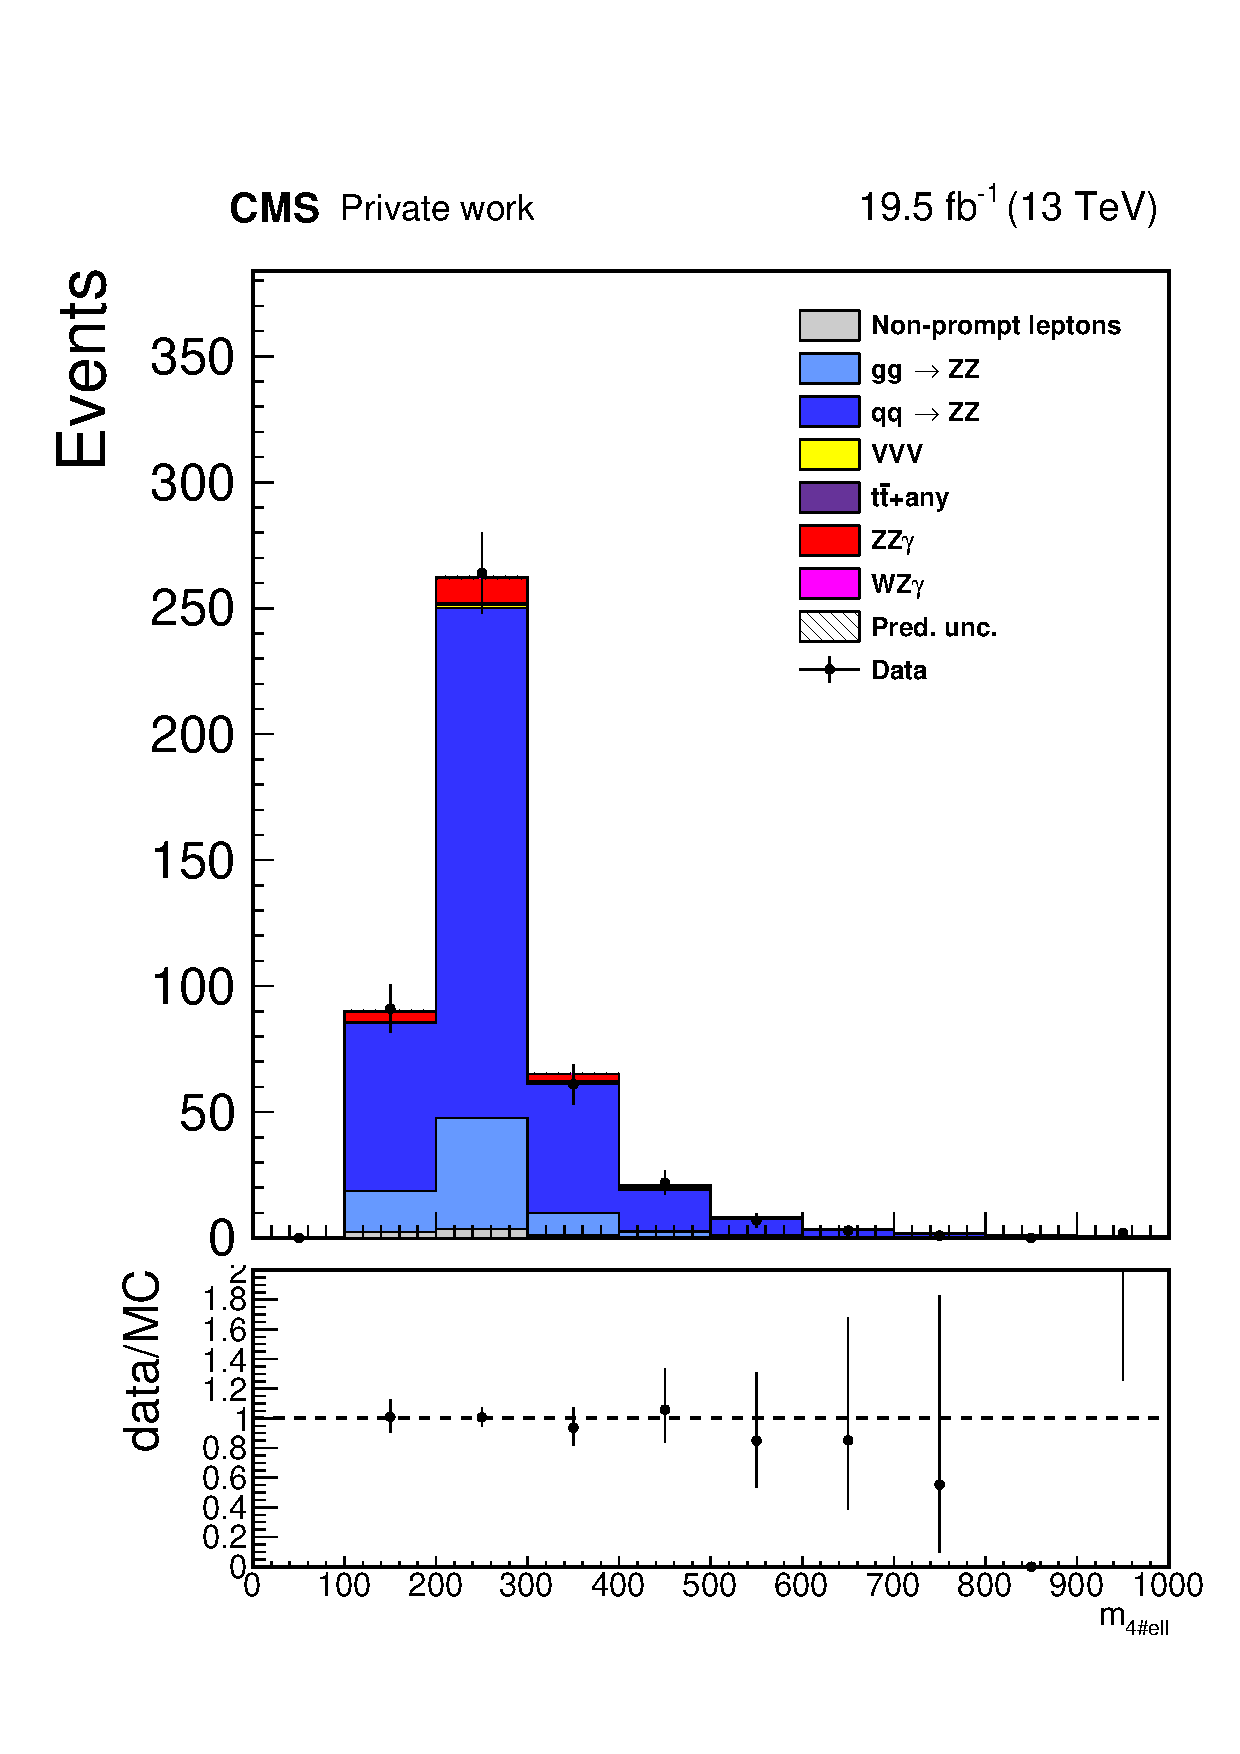
\includegraphics[width=.25\textwidth]{Figures/VVGammaAnalyzer/2016preVFP/lepCR/SR4P/ZZ_mass_pow.pdf}}%
\subfigure [2016postVFP] {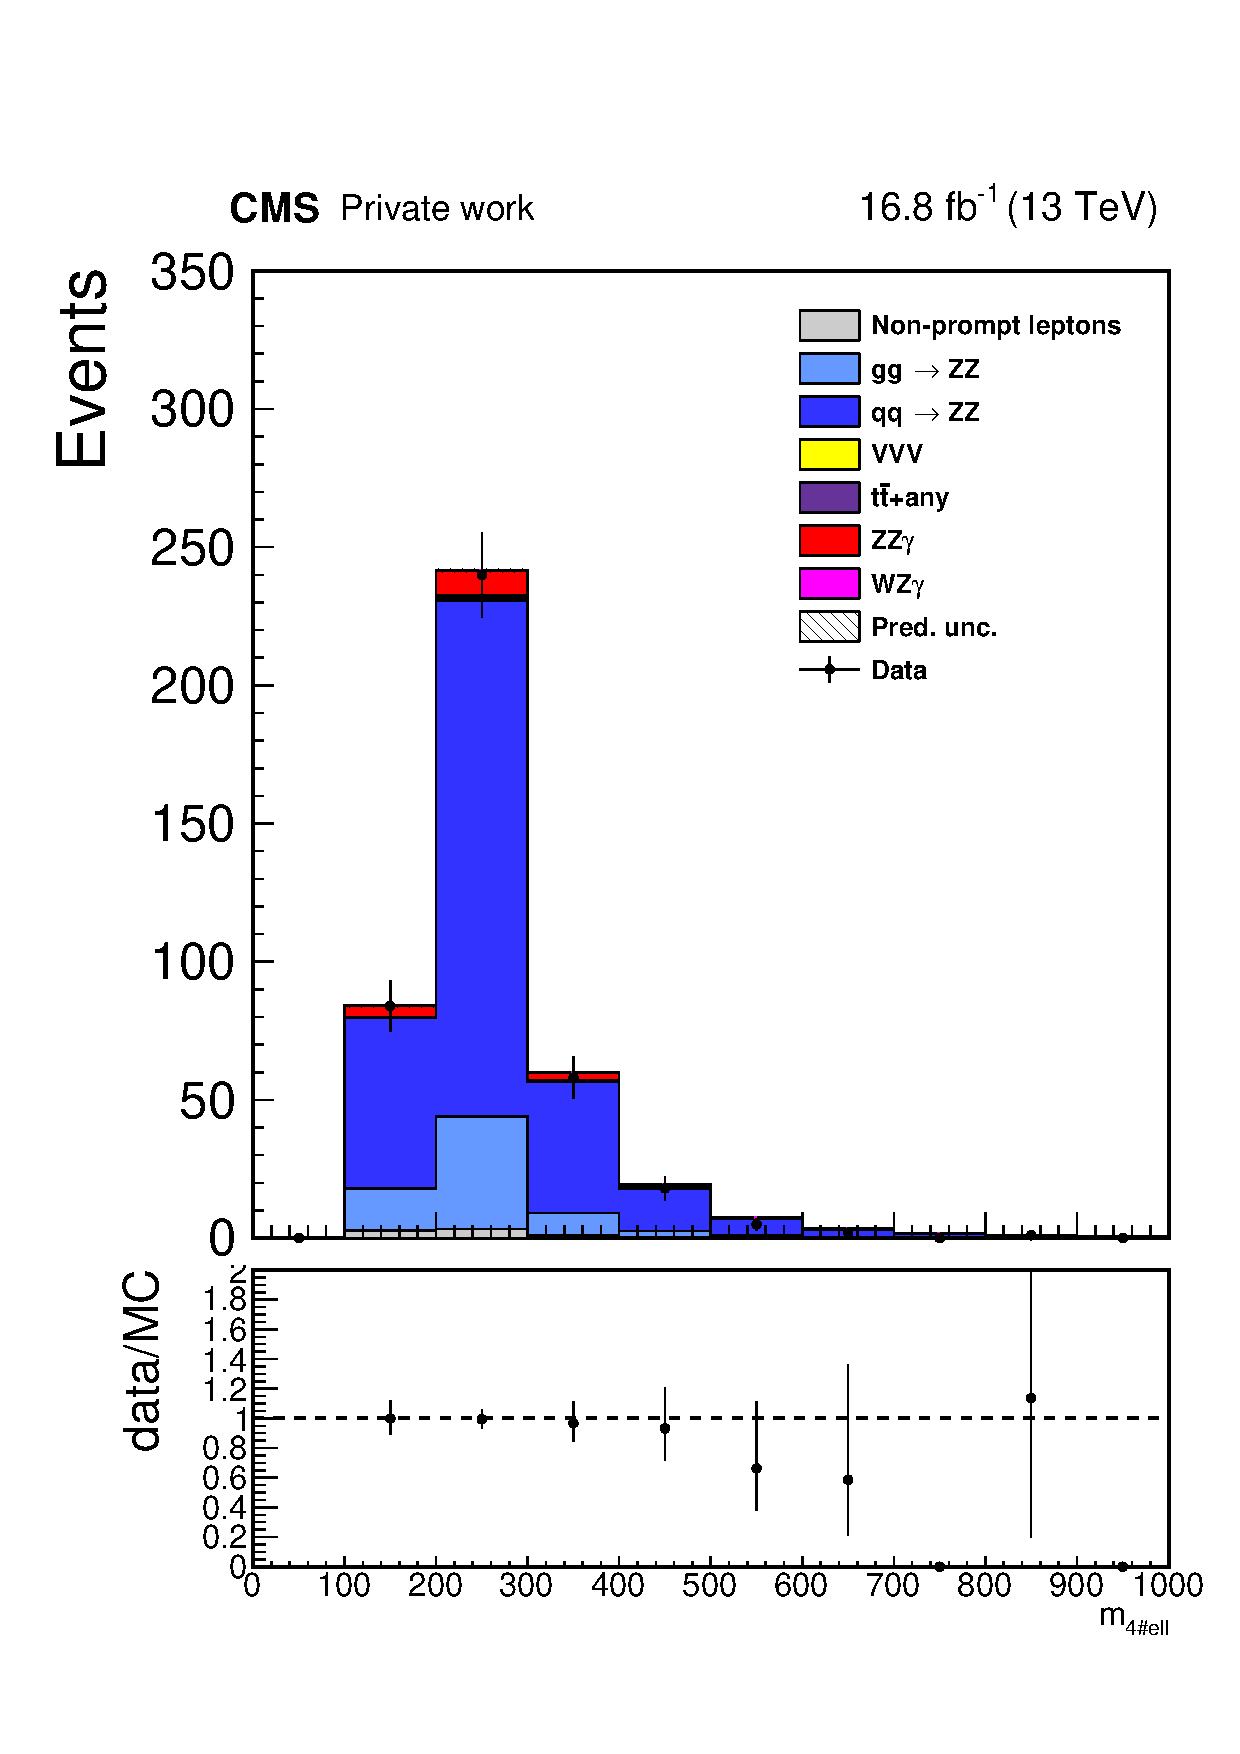
\includegraphics[width=.25\textwidth]{Figures/VVGammaAnalyzer/2016postVFP/lepCR/SR4P/ZZ_mass_pow.pdf}}%
\subfigure [2017       ] {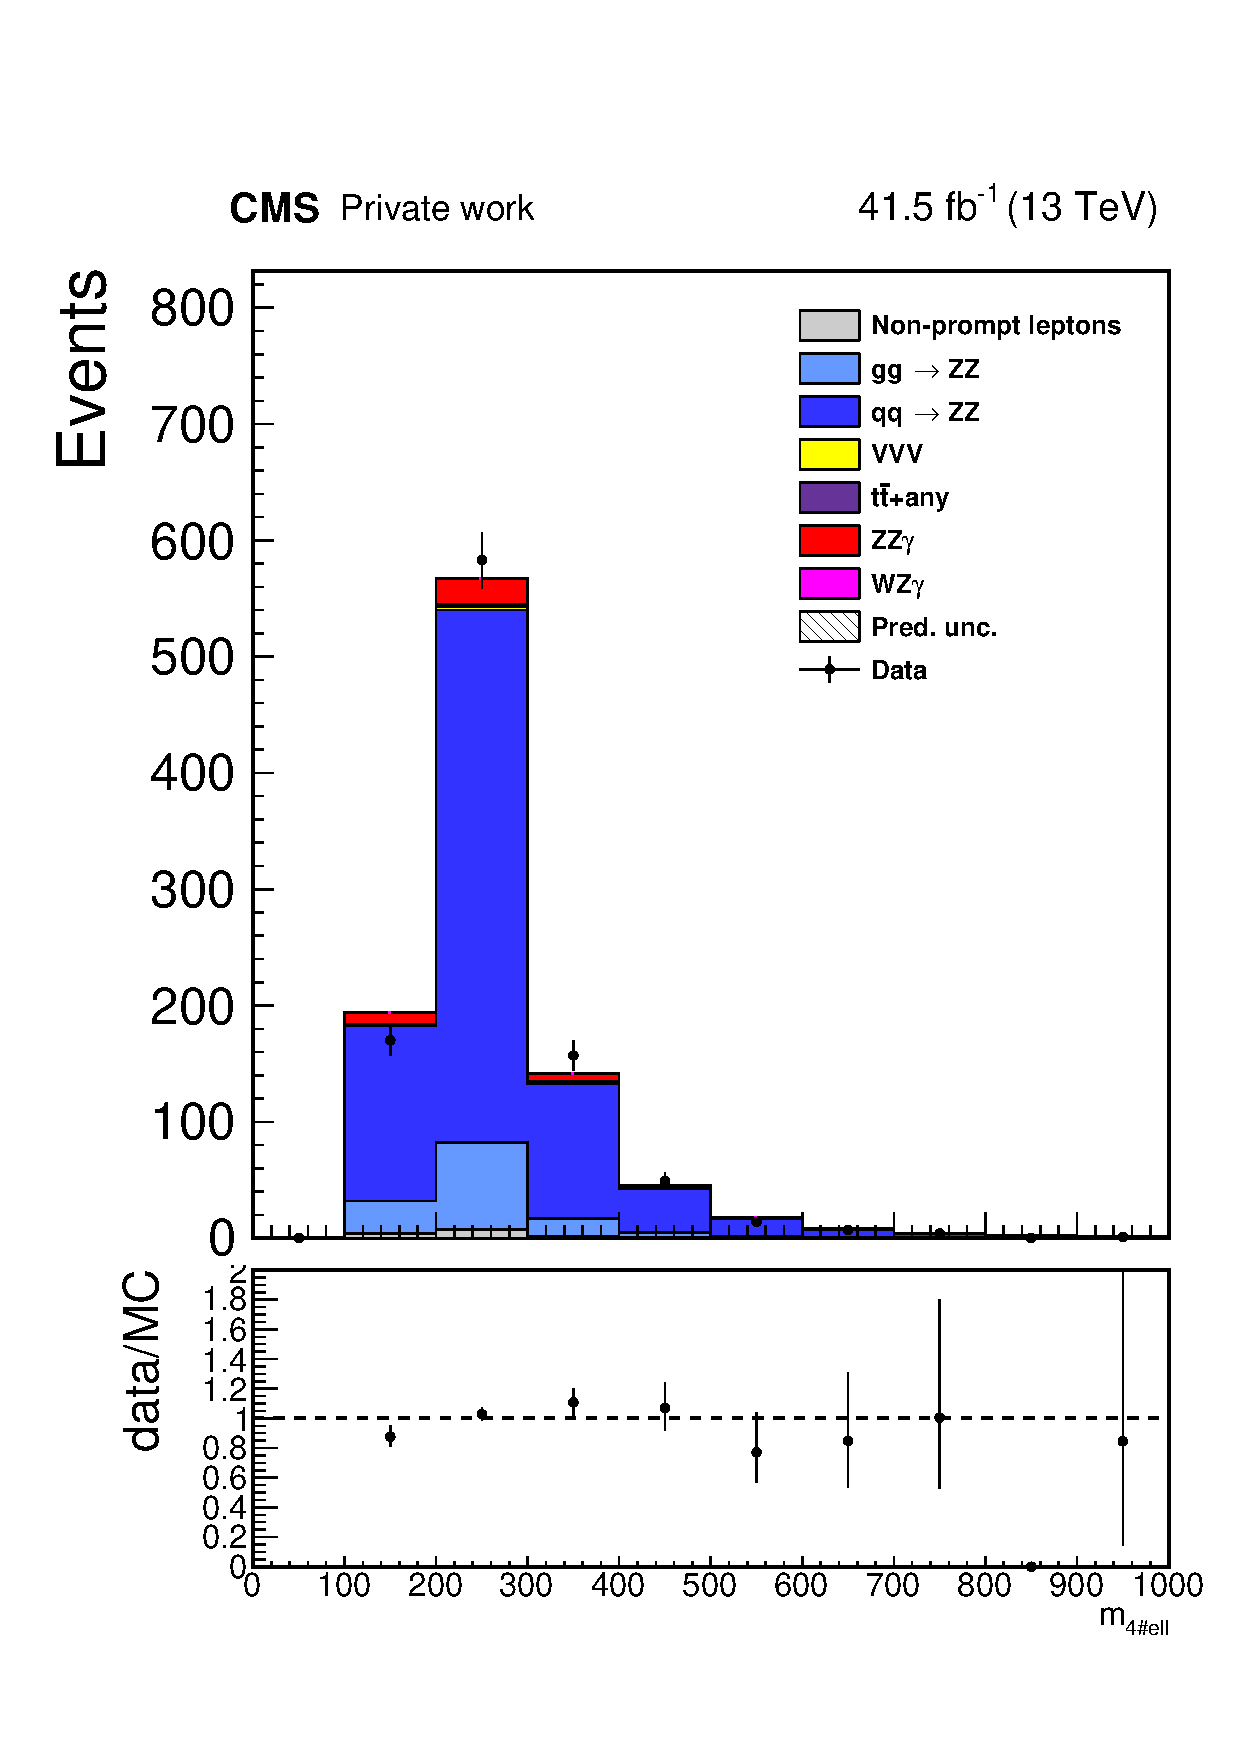
\includegraphics[width=.25\textwidth]{Figures/VVGammaAnalyzer/2017/lepCR/SR4P/ZZ_mass_pow.pdf}}%
\subfigure [2018       ] {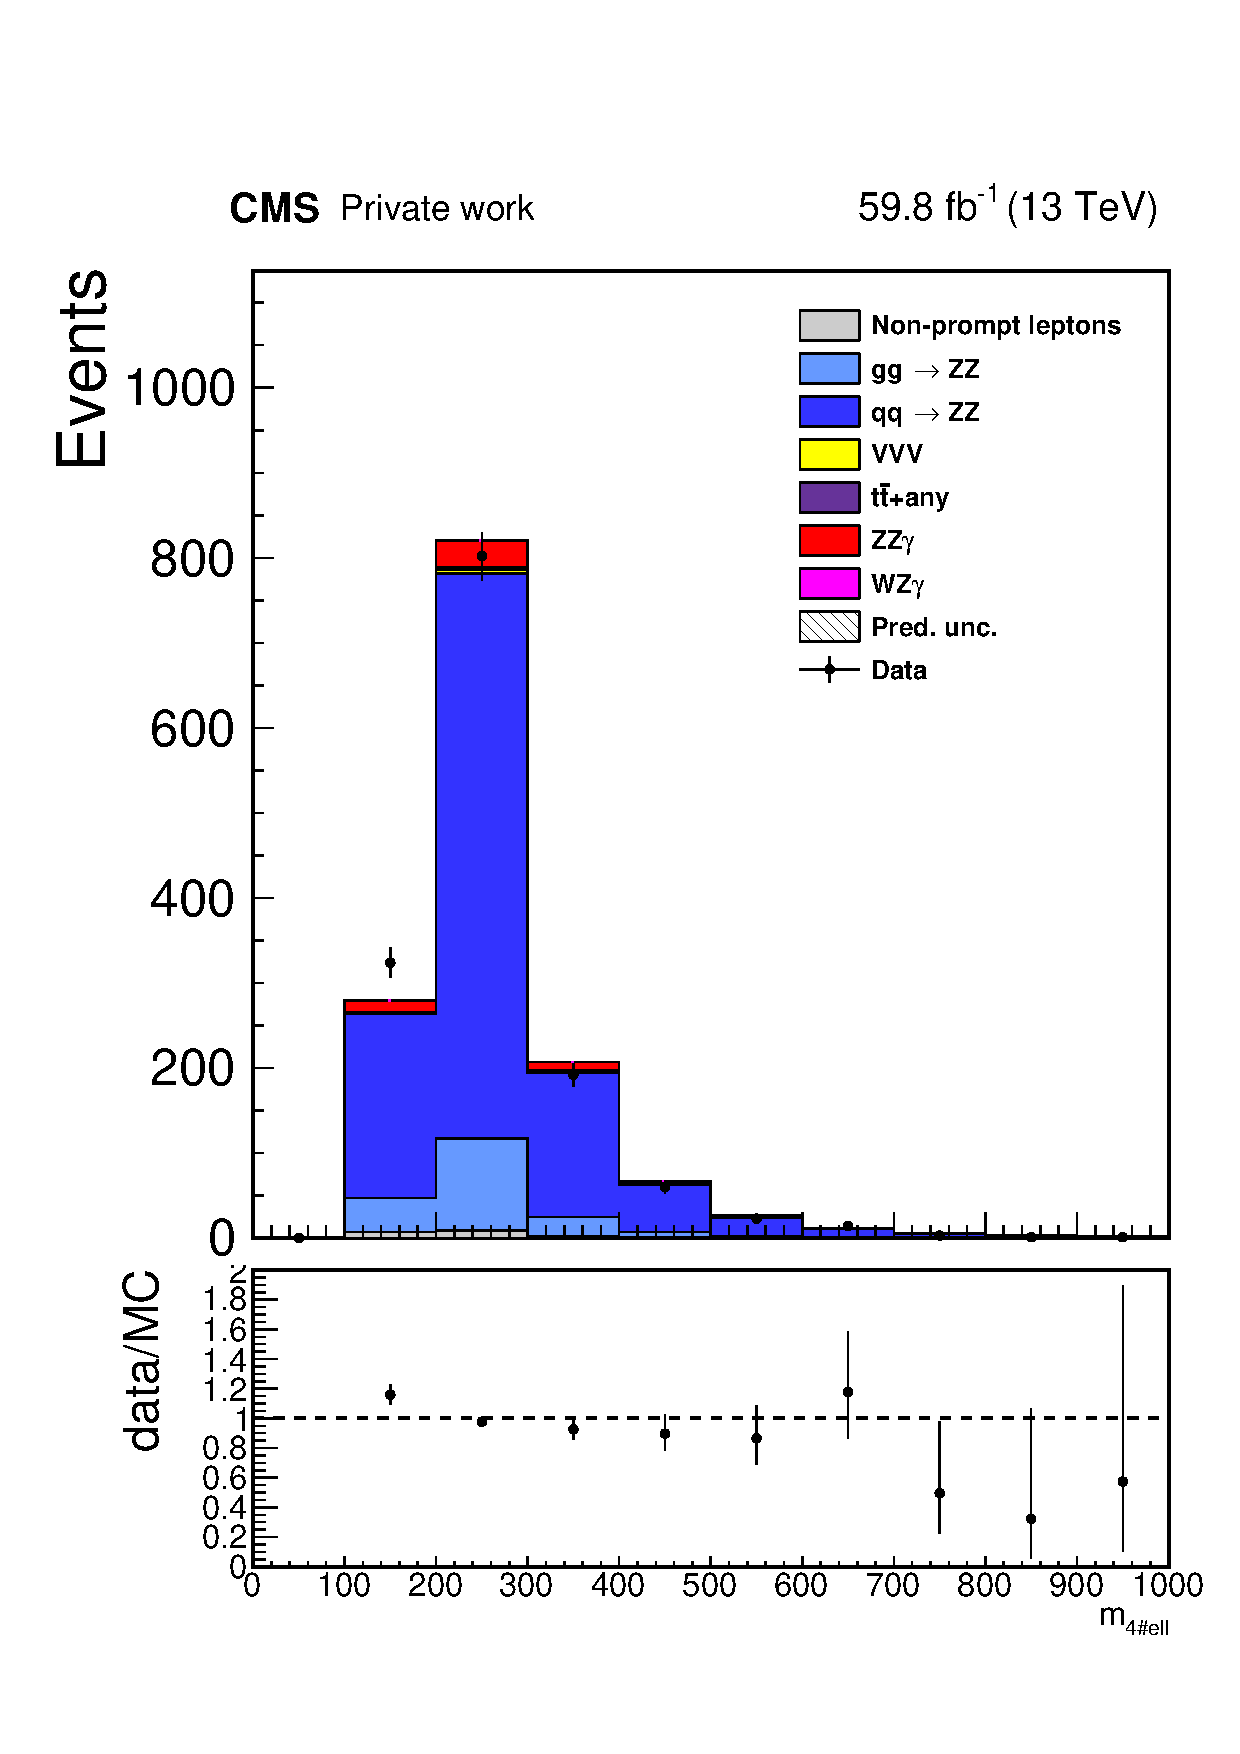
\includegraphics[width=.25\textwidth]{Figures/VVGammaAnalyzer/2018/lepCR/SR4P/ZZ_mass_pow.pdf}}
\caption{Invariant mass of the ZZ system, without any requirements on the presence of photons, for each of the data-taking periods of \Run2.}
\label{fig:ZZmass_byyear}
\end{figure}


\section{Statistical analysis}
\label{sec:statistical_analysis}
A statistical analysis is conducted to assess the presence of the signal process in the observed data,
quantify the significance of the excess over background predictions and measure its cross section.
The statistical inference is performed with the \textsc{Combine Tool} software package~\cite{CMS-NOTE-2011-005,CMS-CAT-23-001}.

\providecommand{\poissonpdf}[2]{\ensuremath{ \frac{{#1}^{#2}}{#2!}e^{-#1} }}

\subsection{Likelihood and nuisance parameters}
The likelihood function is defined as the probability density function for a set of parameters of a model
that quantifies the agreement with a certain set of experimental observables (data).
The model adopted for this analysis defines a signal strength modifier $\mu$,
that multiplies the production cross section of the signal process and leaves all the other processes unchanged.
Each independent source of systematic uncertainty described in Section \ref{sec:systematics} is assigned a nuisance parameter $\theta_i$, and the full set is denoted $\vec\theta$.
They are of no direct interest for this analysis, but must be considered in the fitting procedure to extract correct results.
They enter the model through their probability density function $p_i(\tilde{\theta_i}|\theta_i)$,
which is the probability of measuring a certain value of the parameter given that the true value is $\theta_i$.
Furthermore, the expected yields of background, $b$, and signal, $s$, depend on the value of the nuisance parameters.

The global likelihood function is thus defined as:
\begin{equation}
  \label{eq:likelihood_full}
  \Likelihood(data\, |\, \mu, \vec\theta\,) = \prod_c \Likelihood_c(data\, |\, \mu \cdot s(\vec\theta\,) + b(\vec\theta\,)) \cdot \prod_i p_i(\tilde{\theta_i}\, |\, \theta_i)
\end{equation}
where c runs over all the channels, which are the four data-taking periods (2016preVFP, 2016postVFP, 2017, 2018).
The extraction of the signal strength proceeds through the maximization of the complete likelihood function by varying the parameter of interest $\mu$ and the nuisances.
The $\Likelihood_c$ functions are the PDF of the binned distributions in each channel, and are given by the product of Poisson probabilities for every bin $j$ to observe $n_j$ events:
\begin{equation}
  \label{eq:likelihood_bin}
  \Likelihood_c(data\, |\, \mu \cdot s(\vec\theta\,) + b(\vec\theta\,)) =
                       \prod_j \poissonpdf{\left( \mu \cdot s_j(\vec\theta\,) + b_j(\vec\theta\,) \right)}{n_j}
\end{equation}

\subsection{Treatment of nuisance parameters}
Systematics uncertainties can be categorized into two main classes: the ones that affect only the event yield, and those that have an impact also on the shape of the predicted distributions.
Most of the uncertainties of the first class are parametrized with a log-normal distribution:
\begin{equation}
  \label{eq:lnNdef}
  \Probability(\tilde{\theta}\,|\,\theta) = \frac{1}{\sqrt{2 \pi} \text{ln} k} \cdot \frac{1}{\tilde{\theta}} \cdot \text{exp} \left( -\frac{(\text{ln}(\tilde{\theta}/\theta_m))^2}{2 \text{ln}^2 k} \right)
\end{equation}
which is the distribution of a random variable whose logarithm is normally distributed, with mean $\mu$ = $\text{ln}(\theta_m)$ and standard deviation $\sigma$ = $\text{ln}(k)$.
%% where the parameters $theta_s$ and $k$ can be defined in terms of the mean and standard deviation of a normally distributed variable: $\theta_m = e^{\mu}$ and $k = e^{\sigma}$.
The log-normal is used instead of a Gaussian because it enforces the positive-definite normalization for the nuisance modelled, which is usually multiplying an event yield and thus cannot be negative.

The remaining systematics in the first class are those that represent a background coming from a statistically limited control region, such as the fake leptons and photons.
These are dominated by the statistically uncertainty in the control region and are modelled with a Gamma distribution:
\begin{equation}
  \label{eq:gammadef}
  \Probability(\theta\,|\,N\alpha) = \frac{1}{\Gamma(N) \alpha^N} \theta^{N-1} e^{-\theta/\alpha}
\end{equation}
where $N$ is the number of events in the control region, $\theta$ is the average transfer factor and $\Gamma(x)$ is the Gamma function.

The shape uncertainties of the second class are accounted for by interpolating the event fraction for each bin of three histograms:
the one obtained for the central value, and the two obtained by shifting the nuisance parameter up and down by one standard deviation~\cite{CMS-CAT-23-001}.

\subsection{Quantifying an excess}
To quantify the statistical significance of an excess of events over the background-only hypothesis, the following test statistic is used:
\begin{equation}
  \label{eq:test_statistic}
  t_0 = -2\text{ln} \frac {\Likelihood(data\,|\,0,\widehat{\vec{\theta_0}}\,)} {\Likelihood(data\,|\,\hat\mu,\widehat{\vec\theta}_{\hat\mu})}\,,\quad \text{with}\, \hat\mu \ge 0
\end{equation}

The numerator is evaluated under the background-only hypothesis ($\mu$ = 0), and $\widehat{\vec{\theta_0}}$ is the set of values of nuisance parameters that maximizes it under this null hypothesis.
The denominator is evaluated under the alternative signal + background hypothesis,
and the values $\hat{\mu}$ and $\widehat{\vec{\theta}}_{\hat\mu}$
are those that maximize the likelihood in this hypothesis.
This quantity is positive for a signal-like excess ($\mu$ > 0) and becomes 0 in the absence of an excess ($\mu$ = 0).

The significance of an excess is expressed in terms of the local \textit{p-value}, which is the probability to obtain a value of the test statistic $t_0$ greater than or equal to the one observed in experimental data, under the background-only hypothesis:
\begin{equation}
  \label{eq:pvalue}
  p_0 = \Probability(t_0 \ge t_0^{obs}\, |\, \mu = 0)
\end{equation}
That is, $p_0$ is the probability that a local statistical fluctuation of the background yield
is compatible with the observed data in the background only hypothesis,
at least as much as the signal hypothesis.

The p-value is usually expressed as a \textit{significance} $Z$ using the Gaussian one-sided integral:
\begin{equation}
  \label{eq:significance}
  p_0 = \int_Z^\infty \frac{1}{\sqrt{2\pi}}e^{-x^2/2}dx
\end{equation}

The conventional values of $Z$ = 3$\sigma$ and $Z$ = 5$\sigma$, corresponding to p-values of $1.3 \times 10^{-3}$ and $2.8 \times 10^{-7}$, are used to claim evidence for and the discovery of a new phenomenon respectively.


\subsection{Likelihood scans}
\label{sec:likelihood_scans}
The extraction of the signal strength modifier $\mu$ proceeds through the maximization of the likelihood.
%% as described in Section~\ref{sec:statistical_analysis}.
This procedure can be visualized by scanning the likelihood function for several values of the parameter $\mu$
accounting for the systematic uncertainties affecting the measurement.
For each value the best fit value of the nuisance parameters is computed,
and the resulting value of the likelihood is stored.
The corresponding points are then plotted as a function of $\mu$.

Usually the auxiliary quantity $-2\Delta\ln\Likelihood$ (defined as $t_0$ in Equation~\ref{eq:test_statistic})
is used instead of the likelihood itself.
The width of the its profile is linked to the uncertainty on the estimate of $\mu$ from the fit.
More precisely, the set of values $\{ \mu \mid -2\Delta\ln\Likelihood(\mu) < 1 (4) \}$ corresponds to the 68\usep\% (95\usep\%) confidence interval
in the case of a one-dimensional likelihood fit.

This procedure can also be performed by fixing the values of one or more nuisances instead of allowing them to be fitted by the algorithm.
The effect of fixing the value of one or more parameters is a reduction in the overall width of the likelihood shape.
This difference is ascribed to the effect of the \textit{frozen} parameters.

Nuisance parameters are categorized as follows:
\begin{itemize}
\item \textbf{theory:} uncertainties on the QCD scale, proton PDFs and on the value of \alpS;
%% \item \textbf{data-driven:} uncertainties related to the data-driven estimate of fake lepton or fake photon backgrounds;
\item \textbf{luminosity:} the uncertainty on the integrated luminosity corresponding to the data collected by the CMS experiment;
\item \textbf{experimental:} the other experimental uncertainties, such as the lepton or photon efficiency scale factors or the \pileup{} weight,
      including the uncertainty on the data-driven background prediction;
\item \textbf{statistical:} the remaining uncertainty after freezing all of the nuisances.
\end{itemize}

\subsection{Systematic impacts}
\label{sec:systematic_impacts}
The impact of a given source of systematic is defined as the shift $\Delta\mu$ on the signal strength
induced by fixing the corresponding nuisance parameter $\theta_i$ to its $\pm 1 \sigma$ values,
while profiling the other parameters as normal~\cite{CERN-PH-EP-2014-214}.
This is effectively a measure of the correlation between the $i$-th nuisance and the signal strength,
and is useful for determining which nuisances have the largest effect on the uncertainty.


\section{Four lepton channel}
\label{sec:results_4L}
This section reports the results obtained for the four lepton channel, which is the focus of this thesis.

%% \subsection{Comparison of strategies}
\label{sec:strategy_description}
As mentioned in Sections \ref{sec:evt_photon_selection} and \ref{sec:FSR_cut},
different approaches are used to select the photon
and results are reported both with and without the cut suppressing the FSR contribution,
targeting the inclusive process and a photon and triboson production respectively.
Additionally, several event variables are tested for the final fit to the signal strength.

The first is the invariant mass of the $\PZ\PZ\PGg$ system.
It is expected to be higher for triboson events where the photon comes from
initial state radiation or a triple or quartic gauge coupling than for FSR.
Additionally, it is expected to be sensitive to Beyond Standard Model (BSM) contributions, especially in the high-energy tail.

The second variable is the transverse momentum of the photon.
As the $\PZ\PZ\PGg$ mass and the $\PW\PZ\PGg$ transverse mass,
it is presumed to be sensitive to BSM physics in the high-momentum tail.

The third option considered is the MVA-based ID working point passed by the photon.
In each event, the photon passing the highest MVA working point is selected.
Three bins are defined:
\begin{itemize}
\item \makebox[7em][l]{\bf wp80} The photon passes the \texttt{wp80} working point;
\item \makebox[7em][l]{\bf $\mathrm{wp90} \land \mathrm{!wp80}$} The photon passes \texttt{wp90}, but fails \texttt{wp80};
\item \makebox[7em][l]{\bf None} The photon fails \texttt{wp90};
\end{itemize}
The yield of the simulation in each bin is scaled according to the appropriate scale factors (see Section \ref{sec:photonID}).
This distribution is referred to as ``MVA shape''.

The data-driven estimate of the fake lepton background is employed in all cases,
except when using the data-driven \nonprompt photon.
As discussed in Section~\ref{sec:samples_overlap},
only the events from the $\PQq\PAQq \to \PZ\PZ$ sample
that do not contain a prompt generated photon are used,
to avoid double counting with the signal sample $\PZ\PZ\PGg$.
Additionally, when the data-driven estimate of fake photons is employed,
events in $\PQq\PAQq \to \PZ\PZ$ and $\Pg\Pg \to \PZ\PZ$ that do not contain a prompt photon are excluded.

In particular, the following choices of the aforementioned analysis strategy were tested:
\begin{itemize}
\item Data-driven estimate of fake photons,
  using the Loose working point of the cut-based ID to select the signal photon,
  and performing the analysis on the invariant mass spectrum of the $\PZ\PZ\PGg$ system.
\item Fake photon prediction taken from simulation,
  using the Loose working point of the cut-based ID to select the signal photon,
  and performing the analysis on the invariant mass spectrum of the $\PZ\PZ\PGg$ system.
\item Fake photon prediction taken from simulation,
  using the Loose working point of the cut-based ID to select the signal photon,
  and performing the analysis on the transverse momentum distribution of the photon.
\item Fake photon prediction taken from simulation,
  using the \texttt{wp90} working point of the MVA-based ID to select the signal photon,
  and performing the analysis on the invariant mass spectrum of the $\PZ\PZ\PGg$ system.
\item Fake photon prediction taken from simulation,
  using the \texttt{wp90} working point of the MVA-based ID to select the signal photon,
  and performing the analysis on the transverse momentum distribution of the photon.
\item Fake photon prediction taken from simulation,
  using the \texttt{wp80} working point of the MVA-based ID to select the signal photon,
  and performing the analysis on the invariant mass spectrum of the $\PZ\PZ\PGg$ system.
\item Fake photon prediction taken from simulation,
  using the kinematic selection for the photons,
  and classifying events depending on which is the highest MVA working point passed by the photon.
\end{itemize}

First, expected results are derived for each strategy using an Asimov dataset~\cite{Cowan2011},
and the expected significances, signal strength modifiers and impacts of the systematic uncertainties are evaluated.
Then, the best performing strategy is selected and the results are derived using the actual data.

\subsection{Inclusive cross section}
\label{sec:results_4L_inclusive}
The first results pertain the measurement of the inclusive process $\Pp\Pp \to 4\Pl\PGg$ with $\Pl = \Pe,\,\PGm$.
All of the selections detailed in Section~\ref{sec:event_selection} for the four lepton channel are applied,
but the additional cut to suppress FSR is not.

\subsubsection{Significance}
\begin{table}
  \centering
  \caption{Summary of the expected significance of the signal hypothesis %as opposed to the background-only,
    in the inclusive cross section region of the four lepton channel (SR4P\_1P)
    with different strategies for
    photon identification criterion,
    the estimation of the fake photon background
    and choice of observable.}
  \label{tab:summary_significances_inclusive}
  \begin{tabular}{lccc}
    \toprule
    Photon ID                          & \nonprompt \PGg & Variable         & Significance\\
    \midrule
    \multirow{3}{*}{Cut-based (Loose)} & data-driven     & $m_{\PZ\PZ\PGg}$ & 4.54 $\sigma$\\
                                       & simulation      & $m_{\PZ\PZ\PGg}$ & 5.03 $\sigma$\\
                                       & simulation      & $\pt^\PGg$       & 4.93 $\sigma$\\
    \hline
    \multirow{2}{*}{MVA ({\tt wp90})}  & simulation      & $m_{\PZ\PZ\PGg}$ & 5.47 $\sigma$\\
                                       & simulation      & $\pt^\PGg$       & 5.38 $\sigma$\\
    \hline
    MVA ({\tt wp80})                   & simulation      & $m_{\PZ\PZ\PGg}$ & 5.50 $\sigma$\\
    \hline
    Kinematic                          & simulation      & MVA score        & 5.55 $\sigma$\\
    \bottomrule
  \end{tabular}
\end{table}

The expected significances of the various strategies for the identification of the photon and the estimation of the fake photon background
are illustrated in Table~\ref{tab:summary_significances_inclusive}.
The best results are obtained using the MVA ID for the photon, in particular the ``MVA shape''.
The choice of the variable for the fit does not have a large effect.
The cut-based selection results in a significance around 5\usep$\sigma$,
except for the data-driven estimation of the \nonprompt photon background,
while the MVA based ID results in an increase of around 0.5.

The sensitivity is limited by the amount of data, as discussed in Section~\ref{sec:likelihood_scans_inclusive},
which is in agreement with the observation that the various strategies have expected significances approximately in the same range.
Indeed, as reported in Table~\ref{tab:Run2_SR4P_phoCR_lepCR}, the expected yield in the signal region, using the Loose cut-based ID,
is $21.1 \pm 1.2$ events, of which $13.6 \pm 0.2$ from the signal sample.

\subsubsection{Cross section measurement}
\label{sec:unblinded_4L_inclusive}

The likelihood scans and the study of the impact of each systematic uncertainty are performed
using an Asimov dataset, under the hypothesis that the signal strength is exactly 1,
for each of the strategies.
The breakdown of the total uncertainty on the signal strength between various groups of nuisances is
summarized in Table~\ref{tab:scanl_SR4P_inclusive}.

\begin{table}
  \caption{
  Summary of the likelihood scans using the Asimov dataset, meaning that the signal strenght is set to 1,
  in the inclusive cross section region of the four lepton channel,
  highlighting contribution from each of the nuisance parameter groups to the total uncertainty on the signal strength.
  }
  \label{tab:scanl_SR4P_inclusive}
  \small
  \resizebox{\textwidth}{!}{
  \begin{tabular}{>{\bfseries}l >{$}c<{$} >{$}c<{$} >{$}c<{$} >{$}c<{$} >{$}c<{$} >{$}c<{$} >{$}c<{$} >{$}c<{$} >{$}c<{$}}
    \toprule
    Fake photon & $data-driven$   & $   MC      $   & $   MC      $   & $   MC      $   & $   MC      $   & $   MC      $   & $   MC      $ \\
    Fake lepton & $data-driven$   & $data-driven$   & $data-driven$   & $data-driven$   & $data-driven$   & $data-driven$   & $data-driven$ \\
    Photon ID   & $Loose (cut)$   & $Loose (cut)$   & $Loose (cut)$   & $wp90 (MVA) $   & $wp90 (MVA) $   & $wp80 (MVA) $   & $kinematic  $ \\
    Variable    & m_{\PZ\PZ\PGg}  & m_{\PZ\PZ\PGg}  & \pt^\PGg        & m_{\PZ\PZ\PGg}  & \pt^\PGg        & m_{\PZ\PZ\PGg}  & \text{MVAcut} \\
    \midrule
    $\mu$       & 1.00            & 1.00            & 1.00            & 1.00            & 1.00            & 1.00            & 1.00            \\
    total       & {-}0.31/{+}0.36 & {-}0.29/{+}0.35 & {-}0.27/{+}0.32 & {-}0.29/{+}0.34 & {-}0.28/{+}0.34 & {-}0.28/{+}0.33 & {-}0.28/{+}0.33 \\
    \hline
    statistical & {-}0.30/{+}0.35 & {-}0.29/{+}0.34 & {-}0.27/{+}0.32 & {-}0.28/{+}0.33 & {-}0.28/{+}0.33 & {-}0.27/{+}0.32 & {-}0.28/{+}0.33 \\
    theory      & {-}0.00/{+}0.00 & {-}0.01/{+}0.01 & {-}0.02/{+}0.02 & {-}0.01/{+}0.01 & {-}0.01/{+}0.01 & {-}0.01/{+}0.01 & {-}0.01/{+}0.01 \\
    luminosity  & {-}0.02/{+}0.03 & {-}0.02/{+}0.03 & {-}0.02/{+}0.03 & {-}0.02/{+}0.03 & {-}0.01/{+}0.02 & {-}0.02/{+}0.02 & {-}0.02/{+}0.02 \\
    experimental& {-}0.07/{+}0.08 & {-}0.06/{+}0.07 & {-}0.04/{+}0.06 & {-}0.06/{+}0.07 & {-}0.04/{+}0.05 & {-}0.05/{+}0.06 & {-}0.05/{+}0.06 \\
    \bottomrule
  \end{tabular}
  }
\end{table}

% Justify the choice of the strategy
The event yield in the fake photon application region CR4P\_1F is sufficiently large to
ensure stability to the data-driven estimate of this background in the inclusive signal region SR4P\_1P,
as shown in Table~\ref{tab:yields_Run2_CR4P_1F_lepCR}.
This estimation technique has the additional benefit of being independent of the modelling of
\nonprompt photons by the matrix element generator and the parton shower,
which could affect the division of the $\PQq\PAQq \to \PZ\PZ \to 4\Pl$ sample
based on the presence of a generated prompt photon.

For these reasons, it is chosen as reference strategy.
The post-fit event yields in the signal region are reported in Table~\ref{tab:yields_postfit_inclusive_Run2_SR4P}.
The observed (expected) significance of the signal over the background-only hypothesis with the chosen strategy is
$6.09 \usep\sigma$
($4.54 \usep\sigma$).

\begin{figure}
  \renewcommand{\dataMCblind}{}
  \renewcommand{\expobs}{observed}
  \centering
  \includegraphics[height=.33\textheight]{Figures/dataMC/Run2/phoCR/SR4P/SYS_mZZGloose_central_pow\dataMCblind .pdf}
  \hfill
  \includegraphics[height=.33\textheight]{Figures/combine/inclusive/scan_\expobs_Run2_SR4P_phoCR_lepCR_mZZGloose.pdf}
  \caption{\captionScan{mass of the $\PZ\PZ\PGg$ system}{Loose}{cut-based ID}{s}{not }}
  \label{fig:scan_observed_inclusive_Run2_SR4P}
\end{figure}

\begin{figure}
  \renewcommand{\dataMCblind}{}
  \renewcommand{\expobs}{observed}
  \centering
  %% \includegraphics[height=0.33\textheight]{Figures/dataMC/Run2/phoCR/SR4P/SYS_mZZGloose_central_pow\dataMCblind .pdf}
  %% \hfill
  \includegraphics[height=0.33\textheight]{Figures/combine/inclusive/impacts_\expobs_Run2_SR4P_phoCR_lepCR_mZZGloose.pdf}
  \caption{\captionImpact{mass of the $\PZ\PZ\PGg$ system}{Loose}{cut-based ID}{s}{not }}
  \label{fig:impacts_observed_inclusive_Run2_SR4P}
\end{figure}

\begin{table}
  \caption{Post-fit yields in the inclusive signal region in the four lepton channel
  using the Loose working point of the cut-based ID to select the photon,
  and employing the data-driven estimate of the \nonprompt photon background.}
  \label{tab:yields_postfit_inclusive_Run2_SR4P}
  \centering
  \small
  \providecommand{\headcell}[1]{\text{#1}} %{\makecell[c]{\text{#1}}}
  \resizebox{\textwidth}{!}{
  \begin{tabular}{>{$}l<{$} >{$}c<{$} >{$}c<{$} >{$}c<{$} >{$}c<{$} >{$}c<{$} >{$}c<{$}}
    \toprule
    \text{Process} & \headcell{2016postVFP} & \headcell{2016preVFP} & \headcell{2017} & \headcell{2018} & \headcell{\Run2} \\
    \midrule
    \PZ\PZ\PGg\to4\Pl\PGg       & 2.34 \pm 0.65 & 2.68 \pm 0.74 & 5.48 \pm 1.53 & 7.99 \pm 2.20 & 18.49 \pm 2.85 \\
    \text{Fake photons}         & 0.95 \pm 0.37 & 1.27 \pm 0.50 & 1.16 \pm 0.41 & 2.18 \pm 0.70 & 5.57 \pm 1.02 \\
    \Pg\Pg\to\PZ\PZ\to2\Pe2\PGm & 0.06 \pm 0.00 & 0.06 \pm 0.00 & 0.07 \pm 0.00 & 0.10 \pm 0.01 & 0.29 \pm 0.01 \\
    \Pg\Pg\to\PZ\PZ\to4\Pe      & 0.03 \pm 0.00 & 0.03 \pm 0.00 & 0.07 \pm 0.01 & 0.10 \pm 0.01 & 0.24 \pm 0.01 \\
    \Pg\Pg\to\PZ\PZ\to4\PGm     & 0.05 \pm 0.00 & 0.06 \pm 0.00 & 0.12 \pm 0.00 & 0.16 \pm 0.01 & 0.38 \pm 0.01 \\
    \PQt\PAQt\PZ\text{+jets}    & 0.01 \pm 0.00 & 0.01 \pm 0.00 & 0.04 \pm 0.01 & 0.04 \pm 0.01 & 0.10 \pm 0.02 \\
    \PW\PW\PZ                   & 0.04 \pm 0.01 & 0.00 \pm 0.00 & 0.04 \pm 0.01 & 0.08 \pm 0.01 & 0.16 \pm 0.01 \\
    \PW\PZ\PZ                   & 0.01 \pm 0.01 & 0.00 \pm 0.00 & 0.02 \pm 0.01 & 0.06 \pm 0.01 & 0.08 \pm 0.02 \\
    \noalign{\vspace{.3ex}}\hline\noalign{\vspace{.3ex}}
    \text{Total signal}         & 2.34 \pm 0.65 & 2.68 \pm 0.74 & 5.48 \pm 1.53 & 7.99 \pm 2.20 & 18.49 \pm 2.85 \\
    \text{Total background}     & 1.15 \pm 0.38 & 1.44 \pm 0.50 & 1.53 \pm 0.41 & 2.75 \pm 0.70 & 6.87 \pm 1.02 \\
    \noalign{\vspace{.3ex}}\hline\noalign{\vspace{.3ex}}
    \text{Total}                & 3.49 \pm 0.74 & 4.12 \pm 0.92 & 7.02 \pm 1.58 & 10.73 \pm 2.27 & 25.36 \pm 3.01 \\
    \text{Data}                 & 4 & 3 & 6 & 11 & 24 \\
    \bottomrule
  \end{tabular}
  }
\end{table}

The maximum likelihood fit to the distribution of $m_{4\Pl\PGg}$ results in a signal strength of
$1.38{}^{+0.54}_{-0.47}\stat {}^{+0.01}_{-0.01}\thy {}^{+0.05}_{-0.03}\lum {}^{+0.12}_{-0.10}\syst = 1.38{}^{+0.55}_{-0.48}$,
as shown in Figure~\ref{fig:scan_observed_inclusive_Run2_SR4P}.
The detailed breakdown of each source of systematic uncertainty is reported in
Figure~\ref{fig:impacts_observed_inclusive_Run2_SR4P}.

The signal sample, which includes tau leptons in the final state,
has a cross section of $(22.02 \pm 0.02) \usep\text{fb}$, as reported in Table~\ref{tab:listofsamples}.
Assuming that $\mathcal{B}(\PZ\to2\Pe) = \mathcal{B}(\PZ\to2\PGm) = \mathcal{B}(\PZ\to2\PGt)$
and that the difference in the phase space due to the different mass of the leptons is negligible,
it follows that $\frac{4}{9}$ of the events in the sample have a final state with four among electrons and muons,
while $\frac{1}{9}$ contain four tau leptons and $\frac{4}{9}$ contain two tau leptons and two electrons or muons.
Therefore the $\mathcal{B}(\PZ_0,\PZ_1\to4\Pl)\times\sigma$, with $\Pl = \Pe, \PGm$, of the sample is $(9.787 \pm 0.009)\usep\text{fb}$.

Using the obtained signal strength, the measured cross section for the production of
$\Pp\Pp \to 4\Pl\PGg$ ($\Pl = \Pe,\,\PGm$) at a centre-of-mass energy of $13\TeV$ is \\
$13.52 {}^{+5.24}_{-4.55}\stat {}^{+0.05}_{-0.05}\thy {}^{+0.45}_{-0.31}\lum {}^{+1.15}_{-0.93}\syst \usep\text{fb} = 13.52{}^{+5.38}_{-4.66} \usep\text{fb}$.

The expected results for the other strategies, using the Asimov dataset,
are reported in Appendix~\ref{sec:expected_4L_inclusive}.


\subsection{Triboson fiducial region}
\label{sec:results_4L_FSRcut}
The following results are derived after the application of the cut
designed to suppress FSR and enhance the fraction of events from triboson production diagrams,
described in Section~\ref{sec:FSR_cut}.
The target is the process $\Pp\Pp \to \PZ\PZ\PGg \to 4\Pl\PGg$.

\subsubsection{Significance}
The significances obtained with the various strategies for the identification of the photon
and the estimation of the fake photon background are illustrated in
Table~\ref{tab:summary_significances_FSRcut}.
\begin{table}
  \centering
  \caption{Summary of the expected significance of the signal hypothesis %as opposed to the background-only,
    in the triboson fiducial section region of the four lepton channel (SR4P fiducial)
    with different strategies for
    the estimation of the fake photon background,
    photon identification criterion
    and choice of observable.
  }
  \label{tab:summary_significances_FSRcut}
  \begin{tabular}{lccc}
    \toprule
    Photon ID                          & \nonprompt \PGg & Variable         & Significance\\
    \midrule
    \multirow{3}{*}{Cut-based (Loose)} & data-driven     & $m_{\PZ\PZ\PGg}$ & 4.08 $\sigma$\\
                                       & simulation      & $m_{\PZ\PZ\PGg}$ & 2.98 $\sigma$\\
                                       & simulation      & $\pt^\PGg$       & 2.98 $\sigma$\\
    \hline
    \multirow{2}{*}{MVA ({\tt wp90})}  & simulation      & $m_{\PZ\PZ\PGg}$ & 3.37 $\sigma$\\
                                       & simulation      & $\pt^\PGg$       & 3.34 $\sigma$\\
    \hline
    MVA ({\tt wp80})                   & simulation      & $m_{\PZ\PZ\PGg}$ & 3.56 $\sigma$\\
    \hline
    Kinematic                          & simulation      & MVA score        & 3.48 $\sigma$\\
    \bottomrule
  \end{tabular}
\end{table}


The highest sensitivity is expected with
the MVA score, using the data-driven method only for fake leptons and the simulation for the nonprompt photons.
The second best results are expected with the fit to the invariant mass of the $\PZ\PZ\PGg$ system,
selecting the photon with the \texttt{wp80} of the MVA ID.
The \texttt{wp90} (either $m_{\PZ\PZ\PGg}$ or $\pt^\PGg$) follows,
and the cut-based ID has the worst expected result.

The expected significance is below $3\usep\sigma$ for the cut-based selection,
except when using the data-driven estimate for \nonprompt photons,
while the MVA based selection results in 3.3--3.5\usep$\sigma$.
This region is heavily affected by the low event yield,
with only $6.8 \pm 0.2$ events expected with the cut-based photon ID,
of which $5.6 \pm 0.1$ from the signal sample,
as shown in Table~\ref{tab:yield_SR4P_1P_FSRcut_Loose}.

\subsubsection[Search for triboson ZZgamma production]{Search for triboson $\PZ\PZ\PGg$ production}
\label{sec:unblinded_4L_FSRcut}

As for the inclusive region, likelihood scans are performed for each of the candidate strategies,
and a summary is shown in Table~\ref{tab:scanl_SR4P_FSRcut}.
The full results, including the impacts of each systematic uncertainty, are reported in Appendix~\ref{sec:expected_4L_FSRcut}.

\begin{table}
  \caption{
    Summary of the likelihood scans for the four lepton channel
    in the triboson fiducial region
    and contribution from each of the nuisance parameter groups to the total uncertainty on the signal strength.
  }
  \label{tab:scanl_SR4P_FSRcut}
  \small
  \resizebox{\textwidth}{!}{
  \begin{tabular}{lccccccccc}
    \toprule
    Fake photon & data-driven    &    MC          &    MC         &    MC          &    MC         &    MC          &    MC         \\
    Fake lepton & data-driven    & data-driven    & data-driven   & data-driven    & data-driven   & data-driven    & data-driven   \\
    Photon ID   & Loose (cut)    & Loose (cut)    & Loose (cut)   & wp90 (MVA)     & wp90 (MVA)    & wp80 (MVA)     & kinematic     \\
    Variable    &$m_{\PZ\PZ\PGg}$&$m_{\PZ\PZ\PGg}$& $\pt^\PGg$    &$m_{\PZ\PZ\PGg}$& $\pt^\PGg$    &$m_{\PZ\PZ\PGg}$& MVAcut        \\
    \midrule
    $\mu$       & 1.000000       & 1.000000       & 1.000000      & 1.000000       & 1.000000      & 1.000000       & 1.000000      \\
    total       & -0.424/+0.513  & -0.425/+0.503  & -0.431/+0.514 & -0.406/+0.480 & -0.414/+0.493  & -0.415/+0.496  & -0.404/+0.476 \\
    \hline
    data-driven & -0.037/+0.078  & -0.001/+0.001  & -0.001/+0.001 & -0.001/+0.001  & -0.001/+0.001 & -0.001/+0.001  & -0.002/+0.002 \\
    luminosity  & -0.026/+0.046  & -0.028/+0.043  & -0.028/+0.043 & -0.027/+0.041  & -0.027/+0.042 & -0.026/+0.040  & -0.031/+0.047 \\
    theory      & -0.030/+0.031  & -0.042/+0.040  & -0.040/+0.038 & -0.037/+0.034  & -0.037/+0.035 & -0.034/+0.031  & -0.050/+0.056 \\
    syst        & -0.043/+0.081  & -0.053/+0.080  & -0.052/+0.080 & -0.050/+0.076  & -0.050/+0.076 & -0.048/+0.072  & -0.065/+0.095 \\
    stat        & -0.419/+0.498  & -0.419/+0.493  & -0.425/+0.504 & -0.400/+0.471  & -0.409/+0.484 & -0.410/+0.488  & -0.394/+0.461 \\
    \bottomrule
  \end{tabular}
  }
\end{table}

In the triboson fiducial region of the four lepton channel,
the strategy for which the highest sensitivity is expected is
the one that uses the data-driven estimate for \nonprompt photons.
However, it is affected by the large uncertainty due to the small number
of events in the fake photon application region CR4P\_1F.
As shown in Table~\ref{tab:yield_CR4P_1F_FSRcut},
after the additional cut to suppress FSR, is expected to contain only
$22.4 \pm 0.2$ events.

The second best strategy is the fit on $m_{\PZ\PZ\PGg}$ using the
\texttt{wp80} working point of the MVA based identification for the photon.
The post-fit event yields in the signal region are reported in Table~\ref{tab:yields_postfit_FSRcut_Run2_SR4P}.
The observed (expected) significance of the signal over the background-only hypothesis with this strategy is
$3.09 \usep\sigma$
($3.56 \usep\sigma$),
which is above the threshold for evidence, but insufficient to claim the observation.

\begin{figure}
  \renewcommand{\dataMCblind}{}
  \renewcommand{\expobs}{observed}
  \centering
  \includegraphics[height=.33\textheight]{Figures/dataMC/Run2/lepCR/SR4P/SYS_mZZGwp80_central_pow\dataMCblind .pdf}
  \hfill
  \includegraphics[height=.33\textheight]{Figures/combine/FSRcut/scan_\expobs_Run2_SR4P_phoMC_lepCR_mZZGwp80.pdf}
  \caption{\captionScan{mass of the $\PZ\PZ\PGg$ system}{\texttt{wp80}}{MVA ID}{s}{}}
  \label{fig:scan_observed_FSRcut_Run2_SR4P}
\end{figure}

\begin{figure}
  \renewcommand{\dataMCblind}{}
  \renewcommand{\expobs}{observed}
  \centering
  %% \includegraphics[height=0.33\textheight]{Figures/dataMC_FSRcut/Run2/lepCR/SR4P/SYS_mZZGwp80_central_pow\dataMCblind .pdf}
  %% \hfill
  \includegraphics[height=0.33\textheight]{Figures/combine/FSRcut/impacts_\expobs_Run2_SR4P_phoMC_lepCR_mZZGwp80.pdf}
  \caption{\captionImpact{mass of the $\PZ\PZ\PGg$ system}{\texttt{wp80}}{MVA ID}{s}{}}
  \label{fig:impacts_observed_FSRcut_Run2_SR4P}
\end{figure}

\begin{table}
  \caption{Post-fit yields in the triboson fiducial region in the four lepton channel.}
  \label{tab:yields_postfit_FSRcut_Run2_SR4P}
  \centering
  \small
  \providecommand{\headcell}[1]{\text{#1}} %{\makecell[c]{\text{#1}}}
  \resizebox{\textwidth}{!}{
  \begin{tabular}{>{$}l<{$} >{$}c<{$} >{$}c<{$} >{$}c<{$} >{$}c<{$} >{$}c<{$} >{$}c<{$}}
    \toprule
    \text{Process} & \headcell{2016postVFP} & \headcell{2016preVFP} & \headcell{2017} & \headcell{2018} & \headcell{\Run2} \\
    \midrule
    \PQt\PAQt\PZ+jets           & 0.01 \pm 0.00 & 0.01 \pm 0.00 & 0.02 \pm 0.01 & 0.01 \pm 0.00 & 0.04 \pm 0.01 \\
    \PW\PZ\PZ                   & 0.01 \pm 0.01 & 0.00 \pm 0.00 & 0.04 \pm 0.01 & 0.03 \pm 0.01 & 0.08 \pm 0.01 \\
    \PZ\PZ\PGg\to4\Pl\PGg       & 0.65 \pm 0.33 & 0.76 \pm 0.38 & 1.60 \pm 0.81 & 2.23 \pm 1.13 & 5.24 \pm 1.48 \\
    \qqZZnonpro                 & 0.07 \pm 0.00 & 0.09 \pm 0.01 & 0.21 \pm 0.01 & 0.29 \pm 0.02 & 0.65 \pm 0.02 \\
    \PZ\PZ\PZ                   & 0.00 \pm 0.00 & 0.00 \pm 0.00 & 0.01 \pm 0.00 & 0.02 \pm 0.01 & 0.04 \pm 0.01 \\
    \Pg\Pg\to\PZ\PZ\to2\Pe2\PGm & 0.01 \pm 0.00 & 0.01 \pm 0.00 & 0.02 \pm 0.00 & 0.02 \pm 0.00 & 0.06 \pm 0.00 \\
    \Pg\Pg\to\PZ\PZ\to4\Pe      & 0.01 \pm 0.00 & 0.01 \pm 0.00 & 0.02 \pm 0.00 & 0.03 \pm 0.00 & 0.06 \pm 0.00 \\
    \Pg\Pg\to\PZ\PZ\to4\PGm     & 0.01 \pm 0.00 & 0.01 \pm 0.00 & 0.03 \pm 0.00 & 0.04 \pm 0.00 & 0.10 \pm 0.00 \\
    \noalign{\vspace{.3ex}}\hline\noalign{\vspace{.3ex}}
    \text{Total signal}         & 0.65 \pm 0.33 & 0.76 \pm 0.38 & 1.60 \pm 0.81 & 2.23 \pm 1.13 & 5.24 \pm 1.48 \\
    \text{Total background}     & 0.11 \pm 0.01 & 0.19 \pm 0.02 & 0.45 \pm 0.04 & 0.51 \pm 0.03 & 1.26 \pm 0.06 \\
    \noalign{\vspace{.3ex}}\hline\noalign{\vspace{.3ex}}
    \text{Total}                & 0.77 \pm 0.33 & 0.95 \pm 0.38 & 2.05 \pm 0.81 & 2.74 \pm 1.13 & 6.51 \pm 1.48 \\
    \text{Data}                 & 1 & 0 & 1 & 5 & 7 \\
    \bottomrule
  \end{tabular}
  }
\end{table}

The maximum likelihood fit in the fiducial triboson region results in a signal strength of
$0.96{}^{+0.53}_{-0.41}$
($0.96 {}^{+0.53}_{-0.41}\stat {}^{+0.01}_{-0.01}\thy {}^{+0.02}_{-0.02}\lum {}^{+0.06}_{-0.04}\syst$),
as displayed in Figure~\ref{fig:scan_observed_FSRcut_Run2_SR4P}.
The detailed breakdown of the sources of systematic uncertainty is reported in
Figure~\ref{fig:impacts_observed_FSRcut_Run2_SR4P}.

As previously discussed, the cross section times branching ratio of the signal sample is
$\sigma^{MC}(\Pp\Pp\to\PZ\PZ\PGg)\times\mathcal{B}(\PZ_0,\PZ_1\to\Pl\Pl) = 9.787\usep\text{fb}$, with $\Pl = \Pe, \PGm$.
Furthermore, the study reported in Section~\ref{sec:signal_genstudy} demonstrates
that the fraction of triboson events for the signal sample in the fiducial region is 52\usep\%.

Using the signal strength obtained from the fit, the measured cross section
for triboson production of $\PZ\PZ\PGg$ in the final state with four leptons, either electrons or muons, and a photon is
$4.90{}^{+2.69}_{-2.08}\usep\text{fb}$
($4.90 {}^{+2.67}_{-2.07}\stat {}^{+0.05}_{-0.06}\thy {}^{+0.12}_{-0.08}\lum {}^{+0.29}_{-0.18}\syst \usep\text{fb}$).


\section{Three lepton channel}
\label{sec:results_3L}
The results reported in this section are the preliminary findings
of the work dedicated to this channel.
The variable chosen for the template fit is the transverse mass of the $\PW\PZ\PGg$ system,
which is defined as:
\begin{equation}
  \label{eq:transverse_mass}
  \mT^2 \mathdefined E^2 - p_z^2 = m^2 + \ptvec^{\:2}
\end{equation}
This quantity is used instead of the invariant mass because only the transverse component of the neutrino momentum is measured,
albeit indirectly through the missing energy.
While it is possible to calculate the z-component of the neutrino momentum assuming that the \PW mass is exactly on the peak,
this would introduce an additional bias with no benefit on the sensitivity.

As discussed in Section~\ref{sec:samples_overlap},
the events that contain a prompt generated photon from the
$\PQq\PAQq\to\PZ\PZ$, $\PW\PZ\to3\Pl\PGn$ and Drell-Yan samples are discarded,
to avoid double counting with the signal samples $\PZ\PZ\PGg$, $\PW\PZ\PGg$ and with $\PZ\PGg$.
When the data-driven estimation of fake photon is employed,
events from the samples $\PQq\PAQq\to\PZ\PZ$, $\Pg\Pg\to\PZ\PZ$, $\PW\PZ\to3\Pl\PGn$ and Drell-Yan
without a prompt generated photon are excluded as well.

The photon is selected using the Loose working point of the cut-based ID.
Two strategies are compared:
\begin{itemize}
\item Data-driven estimate of fake photons,
  using the Loose working point of the cut-based ID to select the signal photon,
  and performing the analysis on the transverse mass spectrum of the $\PW\PZ\PGg$ system.
\item Fake photon and lepton predictions taken from simulation,
  using the Loose working point of the cut-based ID to select the signal photon,
  and performing the analysis on the transverse mass spectrum of the $\PW\PZ\PGg$ system.
\end{itemize}

\subsection{Inclusive cross section}
The following results target the inclusive production of
$\Pp\Pp \to 3\Pl\, \PGnl\, \PGg$, with $\Pl = \Pe, \PGm$.
Thus the cut designed to suppress the contributions from genuine photons from FSR is not applied.

\subsubsection{Significance}
The expected sensitivity for the \RunII{} period
using the data-driven estimate of \nonprompt and misidentified photons is
$3.67 \sigma$,
while the result expected using the prediction from the simulation is
$3.06 \sigma$.
This is consistent with the event yields in Tables~\ref{tab:Run2_SR3P_phoCR_lepCR} and~\ref{tab:Run2_SR3P_phoMC_lepCR},
which show different predictions for the background yields in the signal region.

\subsubsection{Likelihood scans}
The extraction of the signal strength modifier $\mu$ proceeds through the maximisation of the likelihood,
as for the four lepton channel.
This procedure is visualised by plotting the scan of the likelihood function as in the four lepton channel.

An estimate of the contribution of the different groups of nuisances is derived
by sequentially freezing them and the signal strength to the best fit value
and profiling the others.

Four groups of parameters are used in the following results:
\begin{itemize}
\item \textbf{theory:} uncertainties on the QCD scale, proton PDFs and on the value of \alpS;
\item \textbf{data-driven:} uncertainties related to the data-driven estimate of fake lepton or fake photon backgrounds;
\item \textbf{luminosity:} the uncertainty on the integrated luminosity corresponding to the data collected by the CMS experiment;
\item \textbf{others:} remaining experimental uncertainties, such as the lepton or photon efficiency scale factors or the \pileup weight;
\end{itemize}

For the second strategy, in which both fake leptons and photons are estimated from simulation,
the data-driven contribution is obviously null.

\begin{figure}
  \centering
  \includegraphics[height=.33\textheight]{Figures/dataMC/Run2/phoCR/SR3P/SYS_mWZGloose_central_pow_\dataMCblind .pdf}
  \hfill
  \includegraphics[height=.33\textheight]{Figures/combine/inclusive/scan_\expobs_Run2_SR3P_phoCR_lepMC_mWZGloose.pdf}
  \caption{\captionScan{transverse mass of the $\PW\PZ\PGg$ system}{Loose}{cut-based ID}{d}{not }}
  \label{fig:scan_Run2_SR3P_phoCR_lepMC_mWZGloose}
\end{figure}

\begin{figure}
  \centering
  \includegraphics[height=.33\textheight]{Figures/dataMC/Run2/fullMC/SR3P/SYS_mWZGloose_central_pow_\dataMCblind .pdf}
  \hfill
  \includegraphics[height=.33\textheight]{Figures/combine/inclusive/scan_\expobs_Run2_SR3P_phoMC_lepMC_mWZGloose.pdf}
  \caption{\captionScan{transverse mass of the $\PW\PZ\PGg$ system}{Loose}{cut-based ID}{s}{not }}
  \label{fig:scan_Run2_SR4P_phoMC_lepMC_mWZGloose}
\end{figure}

The theory group has the highest impact on the total uncertainty on the signal strength,
accounting for $+0.20/-0.19$ when the data-driven estimate for the \nonprompt photons is used
and $+0.37/-0.38$ when all the backgrounds are estimated from simulation.
The second most impacting group is the statistics, with an uncertainty of
$\pm 0.30$ and $+0.28/-0.27$ respectively.
The first strategy has a total uncertainty of $+0.40/-0.37$,
while for the second it is $+0.48/-0.47$,
around $20\usep\%$ higher.


\subsubsection{Systematic impacts}
\label{sec:impacts_SR3P_inclusive}

\begin{figure}
  \centering
  \includegraphics[height=0.33\textheight]{Figures/dataMC/Run2/phoCR/SR3P/SYS_mWZGloose_central_pow_\dataMCblind .pdf}
  \hfill
  \includegraphics[height=0.33\textheight]{Figures/combine/inclusive/impacts_\expobs_Run2_SR3P_phoCR_lepMC_mWZGloose.pdf}
  \caption{\captionImpact{transverse mass of the $\PW\PZ\PGg$ system}{Loose}{cut-based ID}{d}{not }}
  \label{fig:inclusive_cutID_phoCR_mWZGloose}
\end{figure}

\begin{figure}
  \centering
  \includegraphics[height=0.33\textheight]{Figures/dataMC/Run2/fullMC/SR3P/SYS_mWZGloose_central_pow_\dataMCblind .pdf}
  \hfill
  \includegraphics[height=0.33\textheight]{Figures/combine/inclusive/impacts_\expobs_Run2_SR3P_phoMC_lepMC_mWZGloose.pdf}
  \caption{\captionImpact{transverse mass of the $\PW\PZ\PGg$ system}{Loose}{cut-based ID}{s}{not }}
  \label{fig:inclusive_cutID_phoMC_mWZGloose}
\end{figure}

The largest systematic uncertainty is the QCD scale, which accounts for a shift of
$\approx \pm 0.3$ on the signal strength $\mu$.
\note{I checked, and it is NOT applied to the signal, like I did in June last year for 4L (Gullielmo's comment).
  I'm honestly a bit surprised, but maybe some sample has a large uncertainty (DY? But then why this happens also when using data-driven fake photons?).}
The leading experimental uncertainty is due to the electron efficiency scale factors,
similarly to the four lepton channel.

